\documentclass[a4paper]{article}

\def\npart {IV}
\def\nterm {Lent}
\def\nyear {2018}
\def\nlecturer {A.\ J.\ Scholl}
\def\ncourse {Topics in Number Theory}
\def\nnotready {}

% Imports
\ifx \nextra \undefined
  \usepackage[pdftex,
    hidelinks,
    pdfauthor={Dexter Chua},
    pdfsubject={Cambridge Maths Notes: Part \npart\ - \ncourse},
    pdftitle={Part \npart\ - \ncourse},
  pdfkeywords={Cambridge Mathematics Maths Math \npart\ \nterm\ \nyear\ \ncourse}]{hyperref}
  \title{Part \npart\ - \ncourse}
\else
  \usepackage[pdftex,
    hidelinks,
    pdfauthor={Dexter Chua},
    pdfsubject={Cambridge Maths Notes: Part \npart\ - \ncourse\ (\nextra)},
    pdftitle={Part \npart\ - \ncourse\ (\nextra)},
  pdfkeywords={Cambridge Mathematics Maths Math \npart\ \nterm\ \nyear\ \ncourse\ \nextra}]{hyperref}

  \title{Part \npart\ - \ncourse \\ {\Large \nextra}}
\fi

\author{Lectured by \nlecturer \\\small Notes taken by Dexter Chua}
\date{\nterm\ \nyear}

\usepackage{alltt}
\usepackage{amsfonts}
\usepackage{amsmath}
\usepackage{amssymb}
\usepackage{amsthm}
\usepackage{booktabs}
\usepackage{caption}
\usepackage{enumitem}
\usepackage{fancyhdr}
\usepackage{graphicx}
\usepackage{mathtools}
\usepackage{microtype}
\usepackage{multirow}
\usepackage{pdflscape}
\usepackage{pgfplots}
\usepackage{siunitx}
\usepackage{tabularx}
\usepackage{tikz}
\usepackage{tkz-euclide}
\usepackage[normalem]{ulem}
\usepackage[all]{xy}

\pgfplotsset{compat=1.12}

\pagestyle{fancyplain}
\lhead{\emph{\nouppercase{\leftmark}}}
\ifx \nextra \undefined
  \rhead{
    \ifnum\thepage=1
    \else
      \npart\ \ncourse
    \fi}
\else
  \rhead{
    \ifnum\thepage=1
    \else
      \npart\ \ncourse\ (\nextra)
    \fi}
\fi
\usetikzlibrary{arrows}
\usetikzlibrary{decorations.markings}
\usetikzlibrary{decorations.pathmorphing}
\usetikzlibrary{positioning}
\usetikzlibrary{fadings}
\usetikzlibrary{intersections}
\usetikzlibrary{cd}

\newcommand*{\Cdot}{\raisebox{-0.25ex}{\scalebox{1.5}{$\cdot$}}}
\newcommand {\pd}[2][ ]{
  \ifx #1 { }
    \frac{\partial}{\partial #2}
  \else
    \frac{\partial^{#1}}{\partial #2^{#1}}
  \fi
}

% Theorems
\theoremstyle{definition}
\newtheorem*{aim}{Aim}
\newtheorem*{axiom}{Axiom}
\newtheorem*{claim}{Claim}
\newtheorem*{cor}{Corollary}
\newtheorem*{defi}{Definition}
\newtheorem*{eg}{Example}
\newtheorem*{fact}{Fact}
\newtheorem*{law}{Law}
\newtheorem*{lemma}{Lemma}
\newtheorem*{notation}{Notation}
\newtheorem*{prop}{Proposition}
\newtheorem*{thm}{Theorem}

\renewcommand{\labelitemi}{--}
\renewcommand{\labelitemii}{$\circ$}
\renewcommand{\labelenumi}{(\roman{*})}

\let\stdsection\section
\renewcommand\section{\newpage\stdsection}

% Strike through
\def\st{\bgroup \ULdepth=-.55ex \ULset}

% Maths symbols
\newcommand{\bra}{\langle}
\newcommand{\ket}{\rangle}

\newcommand{\N}{\mathbb{N}}
\newcommand{\Z}{\mathbb{Z}}
\newcommand{\Q}{\mathbb{Q}}
\renewcommand{\H}{\mathbb{H}}
\newcommand{\R}{\mathbb{R}}
\newcommand{\C}{\mathbb{C}}
\newcommand{\Prob}{\mathbb{P}}
\renewcommand{\P}{\mathbb{P}}
\newcommand{\E}{\mathbb{E}}
\newcommand{\F}{\mathbb{F}}
\newcommand{\cU}{\mathcal{U}}
\newcommand{\RP}{\mathbb{RP}}
\newcommand{\CP}{\mathbb{CP}}

\newcommand{\ph}{\,\cdot\,}

\DeclareMathOperator{\sech}{sech}
\DeclareMathOperator{\cosech}{cosech}
\DeclareMathOperator{\cosec}{cosec}

\DeclareMathOperator{\covol}{covol}
\DeclareMathOperator{\vol}{vol}

\let\Im\relax
\let\Re\relax
\DeclareMathOperator{\Im}{Im}
\DeclareMathOperator{\Re}{Re}
\DeclareMathOperator{\im}{im}
\DeclareMathOperator{\image}{image}
\DeclareMathOperator{\Ann}{Ann}

\DeclareMathOperator*{\res}{res}
\DeclareMathOperator{\Res}{Res}
\DeclareMathOperator{\Ind}{Ind}

\DeclareMathOperator{\tr}{tr}
\DeclareMathOperator{\diag}{diag}
\DeclareMathOperator{\rank}{rank}
\DeclareMathOperator{\card}{card}
\DeclareMathOperator{\spn}{span}
\DeclareMathOperator{\adj}{adj}

\DeclareMathOperator{\erf}{erf}
\DeclareMathOperator{\erfc}{erfc}

\DeclareMathOperator{\ord}{ord}
\DeclareMathOperator{\Sym}{Sym}

\DeclareMathOperator{\sgn}{sgn}
\DeclareMathOperator{\orb}{orb}
\DeclareMathOperator{\stab}{stab}
\DeclareMathOperator{\ccl}{ccl}

\DeclareMathOperator{\lcm}{lcm}
\DeclareMathOperator{\hcf}{hcf}

\DeclareMathOperator{\Int}{Int}
\DeclareMathOperator{\id}{id}

\DeclareMathOperator{\betaD}{beta}
\DeclareMathOperator{\gammaD}{gamma}
\DeclareMathOperator{\Poisson}{Poisson}
\DeclareMathOperator{\binomial}{binomial}
\DeclareMathOperator{\multinomial}{multinomial}
\DeclareMathOperator{\Bernoulli}{Bernoulli}
\DeclareMathOperator{\like}{like}

\DeclareMathOperator{\var}{var}
\DeclareMathOperator{\cov}{cov}
\DeclareMathOperator{\bias}{bias}
\DeclareMathOperator{\mse}{mse}
\DeclareMathOperator{\corr}{corr}

\DeclareMathOperator{\otp}{otp}
\DeclareMathOperator{\dom}{dom}

\DeclareMathOperator{\Root}{Root}
\DeclareMathOperator{\supp}{supp}
\DeclareMathOperator{\rel}{rel}
\DeclareMathOperator{\Hom}{Hom}
\DeclareMathOperator{\Aut}{Aut}
\DeclareMathOperator{\Gal}{Gal}
\DeclareMathOperator{\Mat}{Mat}
\DeclareMathOperator{\End}{End}
\DeclareMathOperator{\Char}{char}
\DeclareMathOperator{\ev}{ev}
\DeclareMathOperator{\St}{St}
\DeclareMathOperator{\Lk}{Lk}
\DeclareMathOperator{\disc}{disc}
\DeclareMathOperator{\Isom}{Isom}
\DeclareMathOperator{\length}{length}
\DeclareMathOperator{\energy}{energy}
\DeclareMathOperator{\area}{area}
\DeclareMathOperator{\Syl}{Syl}
\DeclareMathOperator{\cl}{cl}
\DeclareMathOperator{\fix}{fix}

\newcommand{\GL}{\mathrm{GL}}
\newcommand{\SL}{\mathrm{SL}}
\newcommand{\PGL}{\mathrm{PGL}}
\newcommand{\PSL}{\mathrm{PSL}}
\newcommand{\PSU}{\mathrm{PSU}}
\newcommand{\Or}{\mathrm{O}}
\newcommand{\SO}{\mathrm{SO}}
\newcommand{\U}{\mathrm{U}}
\newcommand{\SU}{\mathrm{SU}}

\renewcommand{\d}{\mathrm{d}}
\newcommand{\D}{\mathrm{D}}

\tikzset{->/.style = {decoration={markings,
                                  mark=at position 1 with {\arrow[scale=2]{latex'}}},
                      postaction={decorate}}}
\tikzset{<-/.style = {decoration={markings,
                                  mark=at position 0 with {\arrowreversed[scale=2]{latex'}}},
                      postaction={decorate}}}
\tikzset{<->/.style = {decoration={markings,
                                   mark=at position 0 with {\arrowreversed[scale=2]{latex'}},
                                   mark=at position 1 with {\arrow[scale=2]{latex'}}},
                       postaction={decorate}}}
\tikzset{->-/.style = {decoration={markings,
                                   mark=at position #1 with {\arrow[scale=2]{latex'}}},
                       postaction={decorate}}}
\tikzset{-<-/.style = {decoration={markings,
                                   mark=at position #1 with {\arrowreversed[scale=2]{latex'}}},
                       postaction={decorate}}}

\tikzset{circ/.style = {fill, circle, inner sep = 0, minimum size = 3}}
\tikzset{mstate/.style={circle, draw, blue, text=black, minimum width=0.7cm}}

\definecolor{mblue}{rgb}{0.2, 0.3, 0.8}
\definecolor{morange}{rgb}{1, 0.5, 0}
\definecolor{mgreen}{rgb}{0.1, 0.4, 0.2}
\definecolor{mred}{rgb}{0.5, 0, 0}

\def\drawcirculararc(#1,#2)(#3,#4)(#5,#6){%
    \pgfmathsetmacro\cA{(#1*#1+#2*#2-#3*#3-#4*#4)/2}%
    \pgfmathsetmacro\cB{(#1*#1+#2*#2-#5*#5-#6*#6)/2}%
    \pgfmathsetmacro\cy{(\cB*(#1-#3)-\cA*(#1-#5))/%
                        ((#2-#6)*(#1-#3)-(#2-#4)*(#1-#5))}%
    \pgfmathsetmacro\cx{(\cA-\cy*(#2-#4))/(#1-#3)}%
    \pgfmathsetmacro\cr{sqrt((#1-\cx)*(#1-\cx)+(#2-\cy)*(#2-\cy))}%
    \pgfmathsetmacro\cA{atan2(#2-\cy,#1-\cx)}%
    \pgfmathsetmacro\cB{atan2(#6-\cy,#5-\cx)}%
    \pgfmathparse{\cB<\cA}%
    \ifnum\pgfmathresult=1
        \pgfmathsetmacro\cB{\cB+360}%
    \fi
    \draw (#1,#2) arc (\cA:\cB:\cr);%
}
\newcommand\getCoord[3]{\newdimen{#1}\newdimen{#2}\pgfextractx{#1}{\pgfpointanchor{#3}{center}}\pgfextracty{#2}{\pgfpointanchor{#3}{center}}}

\def\Xint#1{\mathchoice
   {\XXint\displaystyle\textstyle{#1}}%
   {\XXint\textstyle\scriptstyle{#1}}%
   {\XXint\scriptstyle\scriptscriptstyle{#1}}%
   {\XXint\scriptscriptstyle\scriptscriptstyle{#1}}%
   \!\int}
\def\XXint#1#2#3{{\setbox0=\hbox{$#1{#2#3}{\int}$}
     \vcenter{\hbox{$#2#3$}}\kern-.5\wd0}}
\def\ddashint{\Xint=}
\def\dashint{\Xint-}

\DeclareMathOperator\Br{Br}
\renewcommand\G{\mathbb{G}}
\newcommand\A{\mathbb{A}}
\DeclareMathOperator\Cl{\mathrm{Cl}}
\newcommand\ab{\mathrm{ab}}
\newcommand\ur{\mathrm{ur}}
\newcommand\CM{\mathrm{CM}}
\newcommand\sprime{\!{\vphantom{\prod}}'}
\renewcommand\sp{\mathrm{sp}}
\begin{document}
\maketitle
{\small
\setlength{\parindent}{0em}
\setlength{\parskip}{1em}
The ``Langlands programme'' is a far-ranging series of conjectures describing the connections between automorphic forms on the one hand, and algebraic number theory and arithmetic algebraic geometry on the other. In these lectures we will give an introduction to some aspects of this programme.

\subsubsection*{Pre-requisites}
The course will follow on naturally from the Michaelmas term courses \emph{Algebraic Number Theory} and \emph{Modular Forms and L-Functions}, and knowledge of them will be assumed. Some knowledge of algebraic geometry will be required in places.
}
\tableofcontents

\setcounter{section}{-1}
\section{Introduction}
In this course, we shall first give an outline of class field theory. We then look at abelian $L$-functions (Hecke, Tate). We then talk about \emph{non-}abelian $L$-functions, and in particular the Weil--Deligne group and local $L$- and $\varepsilon$-factors.

We then talk about local Langlands for $\GL_n$ a bit, and do a bit of global theory and automorphic forms at the end.

The aim is not to prove everything, because that will take 3 courses instead of one, but we are going to make precise definitions and statements of everything.

\section{Class field theory}
\subsection{Preliminaries}
Class field theory is the study of abelian extensions of local or global fields. Before we can do class field theory, we must first know \emph{Galois} theory.
\begin{notation}
  Let $K$ be a field. We will write $\bar{K}$\index{$\bar{K}$} for a separable closure of $K$, and $\Gamma_K = \Gal(\bar{K}/K)$\index{$\Gamma_K$}. We have
  \[
    \Gamma_K = \lim_{L/K\text{ finite separable}} \Gal(L/K),
  \]
  which is a \term{profinite group}. The associated topology is the \term{Krull topology}.
\end{notation}

Galois theory tells us
\begin{thm}[Galois theory]
  There are bijections
  \begin{align*}
    \left\{\parbox{3cm}{\centering closed subgroups of $\Gamma_K$}\right\} &\longleftrightarrow \left\{\parbox{3cm}{\centering subfields $K \subseteq L \subseteq \bar{K}$}\right\}\\
    \left\{\parbox{3cm}{\centering open subgroups of $\Gamma_K$}\right\} &\longleftrightarrow \left\{\parbox{3cm}{\centering finite subfields $K \subseteq L \subseteq \bar{K}$}\right\}
  \end{align*}
\end{thm}

\begin{notation}
  We write \term{$K^{\ab}$} for the maximal abelian subextension of $\bar{K}$, and then
  \[
    \Gal(K^{\ab}/K) = \Gamma_K^{\ab} = \frac{\Gamma_K}{\overline{[\Gamma_K, \Gamma_K]}}.
  \]
\end{notation}
It is crucial to note that while $\bar{K}$ is unique, it is only unique up to non-canonical isomorphism. Indeed, it has many automorphisms, given by elements of $\Gal(\bar{K}/K)$. Thus, $\Gamma_K$ is well-defined up to conjugation only. On the other hand, the abelianization $\Gamma_K^{\ab}$ \emph{is} well-defined. This will be important in later naturality statements.

\begin{defi}[Non-Archimedean local field]\index{non-Archimedean local field}\index{local field}
  A \emph{non-Archimedean local field} is a finite extension of $\Q_p$ or $\F_p((t))$.
\end{defi}
We can also define Archimedean local fields, but they are slightly less interesting.
\begin{defi}[Archimedean local field]\index{Archimedean local field}
  An Archimedean local field is a field that is $\R$ or $\C$.
\end{defi}

If $F$ is a non-Archimedean local field, then it has a canonical normalized valuation
\[
  v = v_F: F^\times \twoheadrightarrow \Z.
\]
\begin{defi}[Valuation ring]\index{valuation ring}
  The \emph{valuation ring} of a non-Archimedean local field $F$ is
  \[
    \mathcal{O} = \mathcal{O}_F = \{x \in F : v(x) \geq 0\}.
  \]
  Any element $\pi = \pi_f \in \mathcal{O}_F$ with $v(\pi) = 1$ is called a \term{uniformizer}. This generates the maximal idea
  \[
    \mathfrak{m} = \mathfrak{m}_F = \{x \in \mathcal{O}_F: v(x) \geq 1\}.
  \]
\end{defi}

\begin{defi}[Residue field]\index{residue field}
  The \emph{residue field} of a non-Archimedean field $F$ is\index{$k_F$}
  \[
    k = k_F = \mathcal{O}_F/\mathfrak{m}_F.
  \]
  This is a finite field of order $q = p^r$.
\end{defi}

A particularly well-understood subfield of $F^{\ab}$ is the \term{maximal unramified extension} \term{$F^{\ur}$}. We have
\[
  \Gal(F^{\ur}/F) = \Gal(\bar{k}/k) = \hat{\Z} = \lim_{n \geq 1} \Z/n\Z.
\]
and this is completely determined by the behaviour of the residue field. The rest of $\Gamma_F$ is called the \emph{inertia group}.
\begin{defi}[Inertia group]\index{inertia group}\index{$I_F$}
  The \emph{inertia group} $I_F$ is defined to be
  \[
    I_F = \Gal(\bar{F}/F^{\ur}) \subseteq \Gamma_F.
  \]
\end{defi}
We also define
\begin{defi}[Wild inertia group]\index{wild inertia group}\index{$P_F$}
  The \emph{wild inertia group} $P_F$ is the maximal pro-$p$-subgroup of $I_F$.
\end{defi}

Returning to the maximal unramified extension, note that saying $\Gal(\bar{k}/k) \cong \hat{\Z}$ requires picking an isomorphism, and this is equivalent to picking an element of $\hat{\Z}$ to be the ``$1$''. Naively, we might pick the following:
\begin{defi}[Arithmetic Frobenius]\index{arithmetic Frobenius}
  The \emph{arithmetic Frobenius} $\varphi_q \in \Gal(\bar{k}/k)$ (where $|k| = q$) is defined to be
  \[
    \varphi_q(x) = x^q.
  \]
\end{defi}

Identifying this with $1 \in \hat{\Z}$ leads to infinite confusion, and we shall not do so. Instead, we define
\begin{defi}[Geometric Frobenius]\index{geometric Frobenius}
  The \emph{geometric Frobenius} is\index{$\Frob_q$}
  \[
    \Frob_q = \varphi_q^{-1} \in \Gal(\bar{k}/k).
  \]
\end{defi}
We shall identify $\Gal(\bar{k}/k) \cong \hat{\Z}$ by setting the \emph{geometric} Frobenius to be $1$.

The reason this is called the geometric Frobenius is that if we have a scheme over a finite field $k$, then there are two ways the Frobenius can act on it --- either as a Galois action, or as a pullback along the morphism $(-)^q: k \to k$. The latter corresponds to the geometric Frobenius.

We now turn to understand the inertia groups. The point of introducing the wild inertia group is to single out the ``$p$-phenomena'', which we would like to avoid. To understand $I_F$ better, let $n$ be a natural number prime to $p$. As usual, we write\index{$\mu_n(\bar{k})$}
\[
  \mu_n(\bar{k}) = \{\zeta \in \bar{k}: \zeta^n = 1\}.
\]
We also pick an $n$th root of $\pi$ in $\bar{F}$, say $\pi_n$. By definition, this has $\pi_n^n = \pi$.
\begin{defi}[Tame mod $n$ character]\index{tame character}
  The \emph{tame mod $n$ character} is the map $t(n): I_F = \Gal(\bar{F}/F^{ur}) \to \mu_n(\bar{k})$ given by
  \[
    \gamma \mapsto \gamma(\pi_n)/\pi_n \pmod \pi.
  \]
\end{defi}
Note that since $\gamma$ fixes $\pi = \pi_n^n$, we indeed have
\[
  \left(\frac{\gamma(\pi_n)}{\pi_n}\right)^{n} = \frac{\gamma(\pi_n^n)}{\pi_n^n} = 1.
\]
Moreover, this doesn't depend on the choice of $\pi_n$. Any other choice differs by an $n$th root of unity, but the $n$th root of unity lies in $F^{ur}$ since $n$ is prime to $p$. So $\gamma$ fixes it and so it cancels out in the fraction. For the same reason, if $\gamma$ moves $\pi_n$ at all, then this is visible down in $\bar{k}$, since $\gamma$ would have multiplied $\pi_n$ by an $n$th root of unity, and these $n$th roots are present in $\bar{k}$.

Now that everything is canonically well-defined, we can take the limit over all $n$ to obtain a map
\[
  \hat{t}: I_F \to \lim_{(n, p) = 1} \mu_n(\bar{k}) = \prod_{\ell \not= p} \lim_{m \geq 1} \mu_{\ell^m}(\bar{k}) \equiv \prod_{\ell \not= p} \Z_{\ell}(1)(\bar{k}).
\]
This \term{$\Z_{\ell}(1)(\bar{k})$} is the \term{Tate module} of $\bar{k}^{\times}$. This is isomorphic to $\Z_{\ell}$, but not canonically.

\begin{thm}
  $\ker \hat{t} = P_F$.
\end{thm}
Thus, it follows that \term{maximal tamely ramified extension} of $F$, i.e.\ the fixed field of $P_F$ is
\[
  \bigcup_{(n, p) = 1} F^{ur} (\sqrt[n]{\pi}).
\]

Note that $t(n)$ extends to a map $\Gamma_F \to \mu_n$ given by the same formula, but this now depends on the choice of $\pi_n$, and further, it is not a homomorphism, because
\[
  t(n)(\gamma \delta) = \frac{\gamma\delta(\pi_n)}{\pi_n} = \frac{\gamma(\pi_n)}{\pi_n} \gamma \left(\frac{\delta(\pi_n)}{\pi_n}\right) = t(n)(\gamma) \cdot \gamma(t(n)(\delta)).
\]
So this formula just says that $t(n)$ is a $1$-cocycle. Of course, picking another $\pi_n$ will modify $t(n)$ by a coboundary.

\subsection{Local class field theory}
Local class field theory is a (collection of) theorems that describe abelian extensions of a local field. The key takeaway is that finite abelian extensions of $F$ correspond to open finite index subgroups of $F^\times$, but the theorem says a bit more than that:
\begin{thm}[Local class field theory]\index{local class field theory}\leavevmode
  \begin{enumerate}
    \item Let $F$ be a local field. Then there is a continuous homomorphism, the \term{local Artin map}\index{$\Art_F$}\index{Artin map!local}
      \[
        \Art_F: F^\times \to \Gamma_F^{\ab}
      \]
      with dense image characterized by the properties
      \begin{enumerate}
        \item The following diagram commutes:
          \[
            \begin{tikzcd}
              F^{\times} \ar[d, two heads, "v_F"] \ar[r, "\Art_F"] & \Gamma_F^{\ab} \ar[r, two heads] & \Gamma_F/I_F \ar[d, "\sim"]\\
              \Z \ar[rr, hook] & & \hat{\Z}
            \end{tikzcd}
          \]
        \item If $F'/F$ is finite, then the following diagram commutes:
          \[
            \begin{tikzcd}
              (F')^\times \ar[r, "\Art_{F'}"] \ar[d, "N_{F'/F}"] & \Gamma_{F'}^{\ab} = \Gal(F'^{\ab}/F') \ar[d, "\text{restriction}"]\\
              F^\times \ar[r, "\Art_F"] & \Gamma_F^{\ab} = \Gal(F^{\ab}/F)
            \end{tikzcd}
          \]
      \end{enumerate}
    \item Moreover, the \term{existence theorem} says $\Art_F^{-1}$ induces a bijection
      \[
        \left\{\parbox{4cm}{\centering open finite index\\subgroups of $F^\times$}\right\} \longleftrightarrow \left\{\parbox{4cm}{\centering open subgroups of $\Gamma_F^{\ab}$}\vphantom{\parbox{4cm}{open finite index\\subgroups of $F^\times$}}\right\}
      \]
      Of course, open subgroups of $\Gamma_F^{\ab}$ further corresponds to finite abelian extensions of $F$.

    \item Further, $\Art_F$ induces an isomorphism
      \[
        \mathcal{O}_F^\times \overset{\sim}{\to} \im(I_F \to \Gamma_F^{\ab})
      \]
      and this maps $(1 + \pi \mathcal{O}_F)^\times$ to the image of $P_F$. Of course, the quotient $\mathcal{O}_F^\times/(1 + \pi \mathcal{O}_F)^\times \cong k^\times = \mu_\infty(k)$.

    \item Finally, this is functorial, namely if we have an isomorphism $\alpha: F \overset{\sim}{\to} F'$ and extend it to $\bar{\alpha} :\bar{F} \overset{\sim}{\to} \bar{F}'$, then this induces isomorphisms between the Galois groups $\alpha_*: \Gamma_F \overset{\sim}{\to} \Gamma_{F'}$ (up to conjugacy), and $\alpha_*^{\ab} \circ \Art_F = \Art_{F'} \circ \alpha_*^{\ab}$.\fakeqed
  \end{enumerate}
\end{thm}

On the level of finite Galois extensions $E/F$, we can rephrase the first part of the theorem as giving a map
\[
  \Art_{E/F}: \frac{F^\times}{N_{E/F}(E^\times)} \to \Gal(E/F)^{\ab}
\]
which is now an isomorphism (since a dense subgroup of a discrete group is the whole thing!).

We can write down these maps explicitly in certain special cases. We will not justify the following example:
\begin{eg}
  If $F = \Q_p$, then
  \[
    F^{\ab} = \Q_p(\mu_\infty) = \bigcup \Q_p(\mu_n) = \Q_p^{ur} (\mu_{p^\infty}).
  \]
  Moreover, if we write $x \in \Q_p^\times$ as $p^n y$ with $y \in \Z_p^\times$, then
  \[
    \Art_\Q(x)|_{\Q_p^{ur}} = \Frob_p^n,\quad \Art_\Q(x) |_{\Q_p(\mu_{p^\infty})} = (\zeta_{p^n} \mapsto \zeta_{p^n}^{y \text{ mod }p^n}).
  \]
  If we had the arithmetic Frobenius instead, then we would have a $-y$ in the power there, which is less pleasant.
\end{eg}

The cases of the Archimedean local fields are easy to write down and prove directly!
\begin{eg}
  If $F = \C$, then $\Gamma_F = \Gamma_F^{ab} = 1$ is trivial, and the Artin map is similarly trivial. There are no non-trivial open finite index subgroups of $\C^\times$, just as there are no non-trivial open subgroups of the trivial group.
\end{eg}

\begin{eg}
  If $F = \R$, then $\bar{\R} = \C$ and $\Gamma_F = \Gamma_F^{ab} = \Z/2\Z = \{\pm 1\}$. The Artin map is given by the sign map. The unique open finite index subgroup of $\R^\times$ is $\R_{>0}^\times$, and this corresponds to the finite Galois extension $\C/\R$.
\end{eg}

As stated in the theorem, the Artin map has dense image, but is not surjective (in general). To fix this problem, it is convenient to introduce the \emph{Weil group}.
\begin{defi}[Weil group]\index{Weil group}
  Let $F$ be a non-Archimedean local field. Then the \emph{Weil group} of $F$ is the topological group $W_F$ defined as follows:
  \begin{itemize}
    \item As a group, it is
      \[
        W_F = \{\gamma \in \Gamma_F \mid \gamma|_{F^{ur}} = \Frob_q^n\text{ for some }n \in \Z\}.
      \]
      Recall that $\Gal(F^{ur}/F) = \hat{\Z}$, and we are requiring $\gamma|_{F^{ur}}$ to be in $\Z$. In particular, $I_F \subseteq W_F$.
    \item The topology is defined by the property that $I_F$ is an \emph{open} subgroup with the profinite topology. Equivalently, $W_F$ is a fiber product of topological groups
      \[
        \begin{tikzcd}
          W_F \ar[r, hook] \ar[d, two heads] & \Gamma_F \ar[d, two heads]\\
          \Z \ar[r, hook] & \hat{\Z}
        \end{tikzcd}
      \]
      where $\Z$ has the discrete topology.
  \end{itemize}
\end{defi}
Note that $W_F$ is not profinite. It is totally disconnected but not compact.

This seems like a slightly artificial definition, but this is cooked up precisely so that
\begin{prop}
  $\Art_F$ induces an \emph{isomorphism} of topological groups
  \[
    \Art_F^W: F^\times \to W_F^{\ab}.
  \]
  This maps $\mathcal{O}_F^\times$ isomorphically onto the inertia subgroup of $\Gamma_F^{\ab}$.
\end{prop}

In the case of Archimedean local fields, we make the following definitions. They will seem rather ad hoc, but we will provide some justification later.
\begin{itemize}
  \item The Weil group of $\C$ is defined to be $W_\C = \C^\times$, and the Artin map $\Art^W_\R$ is defined to be the identity.
  \item The Weil group of $\R$ is defined the non-abelian group
    \[
      W_\R = \bra \C^\times , \sigma \mid \sigma^2 = -1 \in \C^\times, \sigma z \sigma^{-1} = \bar{z}\text{ for all }z \in \C^\times\ket.
    \]
    This is a (non)-split extension of $\C^\times$ by $\Gamma_\R$,
    \[
      1 \to \C^\times \to W_\R \to \Gamma_\R \to 1,
    \]
    where the last map sends $z \mapsto 0$ and $\sigma \mapsto 1$. This is in fact the unique non-split extension of $\Gamma_\R$ by $\C^\times$ where $\Gamma_\R$ acts on $\C^\times$ in a natural way.

    The map $\Art_\R^W$ is better described by its inverse, which maps
    \begin{align*}
      (\Art_\R^W)^{-1}: W_\R^{\ab} &\overset{\sim}{\longrightarrow} \R^\times\\
      z &\longmapsto z \bar{z}\\
      \sigma &\longmapsto -1
    \end{align*}
\end{itemize}

To understand these definitions, we need the notion of the relative Weil group.
\begin{defi}[Relative Weil group]\index{relative Weil group}
  Let $F$ be a non-Archimedean local field, and $E/F$ Galois but not necessarily finite. We define
  \[
    W_{E/F} = \{\gamma \in \Gal(E^{\ab}/F) : \gamma|_{F^{ur}} = \Frob_q^n, n \in \Z\} = \frac{W_F}{\overline{[W_E, W_E]}}.
  \]
  with the quotient topology.
\end{defi}

The $W_{\bar{F}/F} = W_F$, while $W_{F/F} = W_F^{\ab} = F^\times$ by local class field theory.

Now if $E/F$ is a finite extension, then we have an exact sequence of Galois groups
\[
  \begin{tikzcd}
    1 \ar[r]& \Gal(E^{\ab}/E) \ar[r] & \Gal(E^{\ab}/F) \ar[r] & \Gal(E/F) \ar[r] \ar[d, equals]& 1\\
    1 \ar[r] & W_E^{\ab} \ar[r] \ar[u, hook] & W_{E/F} \ar[r] \ar[u, hook] & \Gal(E/F) \ar[r] & 1.
  \end{tikzcd}
\]
By the Artin map, $W_E^{\ab} = E^\times$. So the relative Weil group is an extension of $\Gal(E/F)$ by $E^\times$. In the case of non-Archimedean fields, we have
\[
  \lim_E E^\times = \{1\},
\]
where the field extensions are joined by the norm map. So $\bar{F}^\times$ is invisible in $W_F = \lim W_{E/F}$. The weirdness above comes from the fact that the separable closures of $\R$ and $\C$ are finite extensions.% Observe that the extension above is characterized by an element of $H^2(\Gal(E/F), E^\times) \simeq \frac{1}{n}\Z/\Z$, and it is in fact $\frac{1}{n}$. We see that this is true also in the case of $\R$.

We are, of course, not going to prove local class field theory in this course. However, we can say something about the proofs. There are a few ways of proving it:
\begin{itemize}
  \item The cohomological method (see Artin--Tate, Cassels--Fr\"ohlich), which only treats the first part, namely the existence of $\Art_K$. We start off with a finite Galois extension $E/F$, and we want to construct an isomorphism
    \[
      \Art_{E/F}: F^\times/N_{E/F}(E^\times) \to \Gal(E/F)^{\ab}.
    \]
    Writing $G = \Gal(E/F)$, this uses the cohomological interpretation
    \[
      F^\times/N_{E/F}(E^\times) = \hat{H}^0(G, E^\times),
    \]
    where $\hat{H}$ is the Tate cohomology of finite groups. On the other hand, we have
    \[
      G^{\ab} = H_1(G, \Z) = \hat{H}^{-2}(G, \Z).
    \]
    The main step is to compute
    \[
      H^2(G, E^\times) = \hat{H}^2(G, E^\times) \cong \tfrac{1}{n}\Z/\Z \subseteq \Q/\Z = H^2(\Gamma_F, \bar{F}^\times).
    \]
    where $n = [E:F]$. The final group $H^2(\Gamma_F, \bar{F}^\times)$ is the \term{Brauer group} $\Br(F)$, and the subgroup is just the kernel of $\Br(F) \to \Br(E)$.

    Once we have done this, we then define $\Art_{E/F}$ to be the cup product with the generator of $\hat{H}^2(G, E^\times)$, and this maps $\hat{H}^{-2}(G, \Z) \to \hat{H}^0(G, E^\times)$. The fact that this map is an isomorphism is rather formal.

    The advantage of this method is that it generalizes to duality theorems about $H^*(G, M)$ for arbitrary $M$, but this map is not at all explicit, and is very much tied to abelian extensions.
  \item Formal group methods: We know that the maximal abelian extension of $\Q_p$ is obtained in two steps --- we can write
    \[
      \Q_p^{\ab} = \Q_p^{ur}(\mu_{p^\infty}) = \Q_p^{ur} (\text{torsion points in }\hat{\G}_m),
    \]
    where $\hat{\G}_m$ is the formal multiplication group, which we can think of as $(1 + \mathfrak{m}_{\bar{\Q}_p})^\times$. This generalizes to any $F/\Q_p$ --- we have
    \[
      F^{\ab} = F^{ur}(\text{torsion points in }\hat{\G}_\pi),
    \]
    where $\hat{\G}_\pi$ is the ``Lubin--Tate formal group''. This is described in Iwasawa's book, and also in a paper of Yoshida's. The original paper by Lubin and Tate is also very readable.

    The advantage of this is that it is very explicit, and when done correctly, gives both the existence of the Artin map and the existence theorem. This also has a natural generalization to non-abelian extensions. However, it does not give duality theorems.
  \item Neukrich's method: Suppose $E/F$ is abelian and finite. If $g \in \Gal(E/F)$, we want to construct $\Art_{E/F}^{-1}(g) \in F^\times/N_{E/F}(E^\times)$. The point is that there is only one possibility, because $\bra g\ket$ is a cyclic subgroup of $\Gal(E/F)$, and corresponds to some cyclic extension $\Gal(E/F')$. We have the following lemma:
    \begin{lemma}
      There is a finite $K/F'$ such that $K \cap E = F'$, so $\Gal(KE/K) \cong \Gal(E/F') = \bra g\ket$. Moreover, $KE/K$ is unramified.
    \end{lemma}
    Let $g'|_E = g$, and suppose $g' = \Frob_{KE/K}^a$. If local class field theory is true, then we have to have
    \[
      \Art_{KE/K}^{-1}(g') = \pi_K^a\pmod{N_{KE/K}(KE^\times)}.
    \]
    Then by our compatibility conditions, this implies
    \[
      \Art_{E/F}^{-1}(g) = N_{K/F}(\pi_K^a) \pmod {N_{E/F}(E^\times)}.
    \]
    The problem is then to show that this does not depend on the choices, and then show that it is a homomorphism. These are in fact extremely complicated. Note that everything so far is just Galois theory. Solving these two problems is then where all the number theory goes in.
  \item When class field theory was first done, we first did \emph{global} class field theory, and deduced the local case from that. No one does that anymore nowadays, since we now have purely local proofs. However, when we try to generalize to the Langlands programme, what we have so far all start with global theorems and then proceed to deduce local results.
\end{itemize}

\subsection{Global class field theory}
We now proceed to discuss global class field theory.
\begin{defi}[Global field]\index{global field}
  A \emph{global field} is a number field or $k(C)$ for a smooth projective absolutely irreducible curve $C/\F_q$, i.e.\ a finite extension of $\F_q(t)$.
\end{defi}
A lot of what we can do can be simultaneously done for both types of global fields, but we are mostly only interested in the case of number fields, and our discussions will mostly focus on those.

\begin{defi}[Place]\index{place}
  Let $K$ be a global field. Then a \emph{place} is a valuation on $K$. If $K$ is a number field, we say a valuation $v$ is a \term{finite place} if it is the valuation at a prime $\mathfrak{p} \lhd \mathcal{O}_K$. A valuation $v$ is an \term{infinite place} if comes from a complex or real embedding of $K$. We write $\Sigma_K$ for the set of places of $K$, and \term{$\Sigma_K^\infty$} and \term{$\Sigma_{K, \infty}$} for the sets of finite and infinite places respectively. We also write \term{$v \nmid \infty$} if $v$ is a finite place, and \term{$v \mid \infty$} otherwise.

  If $K$ is a function field, then all places are are finite, and these correspond to closed points of the curve.
\end{defi}

If $v \in \Sigma_K$ is a place, then there is a completion $K \hookrightarrow K_v$. If $v$ is infinite, then $K_v$ is $\R$ or $\C$, i.e.\ an Archimedean local field. Otherwise, $K_v$ is a non-Archimedean local field.

\begin{eg}
  If $\Q = K$, then there is one infinite prime, which we write as $\infty$, given by the embedding $\Q \hookrightarrow \R$. If $v = p$, then we get the embedding $\Q \hookrightarrow \Q_p$ into the $p$-adic completion.
\end{eg}

\begin{notation}
  If $v$ is a finite place, we write $\mathcal{O}_v \subseteq K_v$ for the valuation ring of the completion.
\end{notation}

Any local field has a canonically normalized valuation, but there is no canonical absolute value. It is useful to fix the absolute value of our local fields. For doing class field theory, the right way to put an absolute value on $K_v$ (and hence $K$) is by
\[
  |x|_v = q_v^{-v(x)},
\]
where
\[
  q_v = \left|\frac{\mathcal{O}_v}{\pi_v \mathcal{O}_v}\right|
\]
is the cardinality of the residue field at $v$. For example, if $K = \Q$ and $v = p$, then $q_v = p$, and $|p|_v = \frac{1}{p}$.

In the Archimedean case, if $K_v$ is real, then we set $|x|$ to be the usual absolute value; if $K_v$ is complex, then we take $|x|_v = x\bar{x} = |x|^2$.

The reason for choosing these normalizations is that we have the following product formula:
\begin{prop}[Product formula]\index{product formula}
  If $x \in K^\times$, then
  \[
    \prod_{v \in \Sigma_K} |x|_v = 1.
  \]
\end{prop}
The proof is not difficult. First observe that it is true for $\Q$, and then show that this formula is ``stable under finite extensions'', which extends the result to all finite extensions of $\Q$.

Global class field theory is best stated in terms of adeles and ideles. We make the following definition:
\begin{defi}[Adele]\index{adele}\index{$\mathbb{A}_K$}
  The \emph{adeles} is defined to be the restricted product
  \[
    \A_K = \prod_v\sprime K_V = \Big\{ (x_v)_{v \in K_v} : x_v \in \mathcal{O}_v \text{ for all but finitely many $v \in \Sigma_K^\infty$}\Big\}.
  \]
  We can write this as $K_\infty \times \hat{K}$ or $\A_{K, \infty} \times \A_K^\infty$, where
  \[
    K_\infty = \A_{K, \infty} = K\otimes_\Q \R = \R^{r_1} \times \C^{r_2}.
  \]
  consists of the product over the infinite places, and
  \[
    \hat{K} = \A_K^\infty = \prod_{v \nmid \infty}\sprime K_V = \bigcup_{S \subseteq \Sigma_K^\infty\text{ finite}} \prod_{v \in S} K_v \times \prod_{v \in \Sigma_K^\infty \setminus S} \mathcal{O}_v.
  \]
  This contains $\hat{\mathcal{O}}_K = \prod_{v \nmid \infty} \mathcal{O}_K$. In the case of a number field, $\hat{\mathcal{O}}_K$ is the profinite completion of $\mathcal{O}_K$. More precisely, if $K$ is a number field then
  \[
    \hat{\mathcal{O}}_K = \lim_{\mathfrak{a}} \mathcal{O}_K/\mathfrak{a} = \lim \mathcal{O}_K/N\mathcal{O}_K = \mathcal{O}_K \otimes_\Z \hat{\Z},
  \]
  where the last equality follows from the fact that $\mathcal{O}_K$ is a finite $\Z$-module.
\end{defi}
%When adeles was first invented, they used the normal product instead of the restricted product, and it turned out to be a terrible idea, since taking the product of infinitely many copies of $\Z$'s lying inside each $K_V$ gives you something ghastly.

\begin{defi}[Idele]\index{idele}\index{$J_K$}\index{$\mathbb{A}_K^\times$}
  The \emph{ideles} is the restricted product
  \[
    J_K = \A_K^\times = \prod_v\sprime K_v^\times = \Big\{(x_v)_v \in \prod K_v^\times: x_v \in \mathcal{O}_v^\times\text{ for almost all } v\Big\}.
  \]
\end{defi}
These objects come with natural topologies. On $\A_K$, we take $K_\infty \times \hat{\mathcal{O}}_K$ to be an open subgroup with the product topology. Once we have done this, there is a unique structure of a topological ring for which this holds. On $J_K$, we take $K_\infty^\times \times \hat{\mathcal{O}}_K^\times$ to be open with the product topology. Note that this is not the subspace topology under the inclusion $J_K \hookrightarrow \A_K$. Instead, it is induced by the inclusion
\begin{align*}
  J_K &\hookrightarrow \A_K \times \A_K\\
  x &\mapsto (x, x^{-1}).
\end{align*}

It is a basic fact that $K^\times \subseteq J_K$ is a \emph{discrete} subgroup.
\begin{defi}[Idele class group]
  The \term{idele class group} is then
  \[
    C_K = J_K/K^\times.
  \]
\end{defi}
The idele class group plays an important role in global class field theory. Note that $J_K$ comes with a natural absolute value
\begin{align*}
  |\ph|_A: J_K &\to \R_{> 0}^\times\\
  (x_v) &\mapsto \prod_{v \in \Sigma_K} |x_v|_v.
\end{align*}
The product formula implies that $|K^\times|_{\A} = \{1\}$. So this in fact a map $C_K \to \R_{>0}^\times$. Moreover, we have

\begin{thm}
  The map $|\ph|_\A: C_K \to \R_{>0}^\times$ has compact kernel.
\end{thm}
This seemingly innocent theorem is actually quite powerful. For example, we will later construct a continuous surjection $C_K \to \Cl(K)$ to the ideal class group of $K$. In particular, this implies $\Cl(K)$ is finite! In fact, the theorem is equivalent to the finiteness of the class group and Dirichlet's unit theorem.

\begin{eg}
  In the case $K = \Q$, we have, by definition,
  \[
    J_{\Q} = \R^\times \times \prod_p\sprime \Q_p^\times.
  \]
  Suppose we have an idele $x = (x_v)$. It is easy to see that there exists a unique rational number $y \in \Q^\times$ such that $\sgn(y) = \sgn(x_\infty)$ and $v_p(y) = v_p(x_p)$. So we have
  \[
    J_\Q = \Q^\times \times \left(\R^\times_{>0} \times \prod_p \Z_p^\times\right).
  \]
  Here we think of $\Q^\times$ as being embedded diagonally into $J_\Q$, and as we have previously mentioned, $\Q^\times$ is discrete. From this description, we can read out a description of the idele class group
  \[
    C_\Q = \R_{>0}^\times \times \hat{\Z}^\times,
  \]
  and $\hat{\Z}^\times$ is the kernel $|\ph|_{\A}$.
\end{eg}

From the decomposition above, we see that $C_\Q$ has a maximal connected subgroup $\R^{\times}_{>0}$. In fact, this is the intersection of all open subgroups containing $1$. For a general $K$, we write \term{$C_K^0$} for the maximal connected subgroup, and then
\[
  \pi_0(C_K) = C_K/C_K^0,
\]
In the case of $K = \Q$, we can naturally identify
\[
  \pi_0(C_\Q) = \hat{\Z}^\times = \lim_n (\Z/n\Z)^\times = \lim_n \Gal(\Q(\zeta_n)/\Q) = \Gal(\Q(\zeta_\infty)/\Q).
\]
The field $\Q(\zeta_\infty)$ is not just any other field. The Kronecker--Weber theorem says this is in fact the maximal abelian extension of $\Q$. Global class field theory is a generalization of this isomorphism to all fields.

Just like in local class field theory, global class field theory involves a certain Artin map. In the local case, we just pulled them out of a hat. To construct the global Artin map, we simply have to put these maps together to form a global Artin map.

Let $L/K$ be a finite Galois extension, $v$ a place of $K$, and $w \mid v$ a place of $L$ extending $v$. For finite places, this means the corresponding primes divide; for infinite places, this means the embedding $w$ is an extension of $v$. We then have the \term{decomposition group}
\[
  \Gal(L_w/K_v) \subseteq \Gal(L/K).
\]
If $L/K$ is abelian, since any two places lying above $v$ are conjugate, this depends only on $v$. In this case, we can now define the \term{global Artin map}\index{Artin map!global}
\begin{align*}
  \Art_{L/K}: J_K &\longrightarrow \Gal(L/K)\\
  (x_v)_v &\longmapsto \prod_v \Art_{L_w/K_v} (x_v),
\end{align*}
where we pick one $w$ for each $v$. To see this is well-defined, note that if $x_v \in \mathcal{O}_v^\times$ and $L/K$ is unramified at $v \nmid \infty$, then $\Art_{K_w/K_v}(x_v) = 1$. So the product is in fact finite.

By the compatibility of the Artin maps, we can passing on to the limit over all extensions $L/K$, and get a continuous map
\[
  \Art_K : J_K \to \Gamma_K^{\ab}.
\]
\begin{thm}[Artin reciprocity law]\index{Artin reciprocity law}\leavevmode
  $\Art_K(K^\times) = \{1\}$, so induces a map $C_K \to \Gamma_K^{\ab}$. Moreover,
  \begin{enumerate}
    \item If $\Char(K) = p > 0$, then $\Art_K$ is injective, and induces an isomorphism $\Art_K: C_k \overset{\sim}{\to} W_K^{\ab}$, where $W_K$ is defined as follows: since $K$ is a finite extension of $\F_q(T)$, and wlog assume $\bar{\F}_q \cap K = \F_q \equiv k$. Then $W_K$ is defined as the pullback
      \[
        \begin{tikzcd}
          W_K \ar[r, hook] \ar[d] & \Gamma_K = \Gal(\bar{K}/K) \ar[d, "\mathrm{restr}."]\\
          \Z \ar[r, hook] & \hat{\Z} \cong \Gal(\bar{k}/k)
        \end{tikzcd}
      \]
    \item If $\Char(K) = 0$, we have an isomorphism
      \[
        \Art_K: \pi_0(C_K) = \frac{C_K}{C_K^0} \overset{\sim}{\to} \Gamma_K^{\ab}.
      \]
  \end{enumerate}
  Moreover, if $L/K$ is finite, then we have a commutative diagram
  \[
    \begin{tikzcd}
      C_L \ar[d, "N_{L/K}"] \ar[r, "\Art_L"] & \Gamma_L^{\ab} \ar[d, "\mathrm{restr.}"]\\
      C_K \ar[r, "\Art_K"] & \Gamma_K^{\ab}
    \end{tikzcd}
  \]
  If this is in fact Galois, then this induces an isomorphism
  \[
    \Art_{L/K}: \frac{J_K}{K^\times N_{L/K}(J_L)} \overset{\sim}{\to} \Gal(L/K)^{\ab}.
  \]
  Finally, this is functorial, namely if $\sigma: K \overset{\sim}{\to} K'$ is an isomorphism, then we have a commutative square
  \[
    \begin{tikzcd}
      C_K \ar[r, "\Art_K"] \ar[d, "\sigma"] & \Gamma_K^{\ab} \ar[d]\\
      C_{K'} \ar[r, "\Art_{K'}"] & \Gamma_{K'}^{\ab}
    \end{tikzcd}
  \]
\end{thm}
Observe that naturality and functoriality are immediate consequences of the corresponding results for local class field theory.

As a consequence of the isomorphism, we have a correspondence
\begin{align*}
  \left\{\parbox{4.2cm}{\centering finite abelian extensions $L/K$}\right\} &\longleftrightarrow \left\{\parbox{4.2cm}{\centering finite index open subgroups of $J_K$ containing $K^\times$}\right\}\\
  L &\longmapsto \ker(\Art_{L/K}: J_K \to \Gal(L/K))
\end{align*}
Note that there exists finite index subgroups that are not open!

Recall that in local class field theory, if we decompose $K_v = \bra \pi\ket \times \mathcal{O}_v^\times$, then the local Artin map sends $\mathcal{O}_v^\times$ to (the image of) the inertia group. Thus an extension $L_w/K_v$ is unramified iff the local Artin map kills of $\mathcal{O}_v^\times$. Globally, this tells us
\begin{prop}
  If $L/K$ is an abelian extension of global fields, which corresponds to the open subgroup $U \subseteq J_K$ under the Artin map, then $L/K$ is unramified at a finite $v \nmid \infty$ iff $\mathcal{O}_v^\times \subseteq U$.
\end{prop}

We can extend this to the infinite places if we make the appropriate definitions. Since $\C$ cannot be further extended, there is nothing to say for complex places.
\begin{defi}[Ramification]\index{ramification!real place}
  If $v \mid \infty$ is a real place of $K$, and $L/K$ is a finite abelian extension, then we say $v$ is ramified if for some (hence all) places $w$ of $L$ above $v$, $w$ is complex.
\end{defi}
The terminology is not completely standard. In this case, Neukrich would say $v$ is inert instead.

With this definition, $L/K$ is unramified at a real place $v$ iff $K_v^\times = \R^\times \subseteq U$. Note that since $U$ is open, it automatically contains $\R^\times_{> 0}$.

We can similarly read off splitting information.
\begin{prop}
  If $v$ is finite and unramified, then $v$ splits completely iff $K_v^\times \subseteq U$.
\end{prop}
\begin{proof}
  $v$ splits completely iff $L_w = K_v$ for all $w \mid v$, iff $\Art_{L_w/K_v}(K_v^\times) = \{1\}$.
\end{proof}

\begin{eg}
  We will use global class field theory to compute all $S_3$ extensions $L/\Q$ which are unramified outside $5$ and $7$.

  If we didn't have global class field theory, then to solve this problem we have to find all cubics whose discriminant are divisible by $5$ and $7$ only, and there is a cubic diophantine problem to solve.

  While $S_3$ is not an abelian group, it is solvable. So we can break our potential extension as a chain
  \begin{center}
    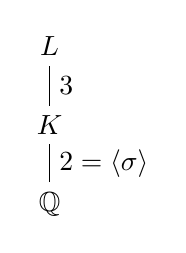
\begin{tikzpicture}
      \node (Q) {$\Q$};
      \node (K) at (0, 1) {$K$};
      \node (L) at (0, 2) {$L$};
      \draw (Q) -- (K) node [pos=0.5, right] {$2 = \bra \sigma\ket$};
      \draw (K) -- (L) node [pos=0.5, right] {$3$};
    \end{tikzpicture}
  \end{center}
  Since $L/\Q$ is unramified outside $5$ and $7$, we know that $K$ must be one of $\Q(\sqrt{5})$, $\Q(\sqrt{-7})$ and $\Q(\sqrt{-35})$. We then consider each case in turn, and then see what are the possibilities for $L$. We shall only do the case $K = \Q(\sqrt{-7})$ here. If we perform similar computations for the other cases, we find that the other choices of $K$ do not work.

  So fix $K = \Q(\sqrt{-7})$. We want $L/K$ to be cylic of degree $3$, and $\sigma$ must act non-trivially on $L$ (otherwise we get an abelian extension).

  Thus, by global class field theory, we want to find a subgroup $U \leq J_K$ of index $3$ such that $\mathcal{O}_v^\times \subseteq U$ for all $v \nmid 35$. We also need $\sigma(U) = U$, or else the composite extension would not even be Galois, and $\sigma$ has to acts as $-1$ on $J_K/U \cong \Z/3\Z$ to get a non-abelian extension.

  We know $K = \Q(\sqrt{-7})$ has has class number $1$, and the units are $\pm 1$. So we know
  \[
    \frac{C_K}{C_K^0} = \frac{\hat{\mathcal{O}}_K^\times}{\{\pm 1\}}.
  \]
  By assumption, we know $U$ contains $\prod_{v \nmid 35} \mathcal{O}_v^\times$. So we have to look at the places that divide $35$. In $\mathcal{O}_{\Q(\sqrt{-7})}$, the prime $5$ is inert and $7$ is ramified.

  Since $5$ is inert, we know $K_5/\Q_5$ is an unramified quadratic extension. So we can write
  \[
    \mathcal{O}_{(5)}^\times = \F_{25}^\times \times (1 + 5\mathcal{O}_{(5)})^\times.
  \]
  The second factor is a pro-5 group, and so it must be contained in $U$ for the quotient to have order $3$. On $\F_{25}^\times$, $\sigma$ acts as the Frobenius $\sigma(x) = x^5$. Since $\F_{25}^\times$ is cyclic of order $24$, there is a unique index $3$ subgroup, cylic of order $6$. This gives an index $3$ sugroup $U_5 \subseteq \mathcal{O}_{(5)}^\times$. Moreover, on here, $\sigma$ acts by $x \mapsto x^5 = x^{-1}$. Thus, we can take
  \[
    U = \prod_{v \not= (5)} \mathcal{O}_v^\times \times U_5,
  \]
  and this gives an $S_3$ extension of $\Q$ that is unramified outside $5$ and $7$. It is an exercise to explicitly identify this extension. % do this

  We turn to the prime $7 = -\sqrt{-7}^2$. Since this is ramified, we have
  \[
    \mathcal{O}_{(\sqrt{-7})}^\times = \F_7^\times \times \left(1 + (\sqrt{-7}) \mathcal{O}_{\sqrt{-7}}\right)^{\times},
  \]
  and again the second factor is a pro-$7$ group. Moreover $\sigma$ acts trivially on $\F_7^\times$. So $U$ must contain $\mathcal{O}_{(\sqrt{-7})}^\times$. So what we found above is the unique such extension.
\end{eg}

We previously explicitly described $C_\Q$ as $\R_{>0}^\times \times \hat{\Z}$. it would be nice to have a similar description of $C_K$ for an arbitrary $K$. The connected component will come from the infinite places $K_\infty^\times \prod_{v \mid \infty} K_v^\times$. The connected component is given by
\[
  K_\infty^{\times, 0} = (\R^\times_{> 0})^{r_1} \times (\C^\times)^{r_2},
\]
where there are $r_1$ real places and $r_2$ complex ones. Thus, we find that
\begin{prop}
  \[
    C_K/C_K^0 = \frac{\{\pm 1\}^{r_1} \times \hat{K}^\times}{\overline{K^\times}}.
  \]
\end{prop}

There is a natural map from the ideles to a more familiar group, called the content homomorphism.
\begin{defi}[Content homomorphism]\index{content homomorphism}
  The \emph{content homomorphism} is the map
  \begin{align*}
    c: J_K&\to \text{ fractional ideals of }K\\
    (x_v)_v &\mapsto \prod_{v \nmid \infty}\mathfrak{p}_v^{v(x_v)},
  \end{align*}
  where $\mathfrak{p}_v$ is the prime ideal corresponding to $v$. We ignore the infinite places completely.
\end{defi}
Observe that $c(K^\times)$ is the set of all principal ideals by definition. Moreover, the kernel of the content map is $K_\infty^\times \times \hat{\mathcal{O}}_K^\times$, by definition. So we have a short exact sequence
\[
  1 \to \frac{\{\pm 1\}^{r_1} \times \hat{\mathcal{O}}_K^\times}{\overline{\mathcal{O}_K^\times}} \to C_K /C_K^0 \to \Cl(K) \to 1.
\]
If $K = \Q $ or $\Q(\sqrt{-D})$, then $\overline{\mathcal{O}_K^\times} = \mathcal{O}_K^\times$ is finite, and in particular is closed. But in general, it will not be closed, and taking the closure is indeed needed.

Returning to the case $K = \Q$, our favorite abelian extensions are those of the form $L = \Q(\zeta_N)$ with $N > 1$. This comes with an Artin map
\[
  \hat{\Z}^\times \cong C_\Q/C_\Q^0 \to \Gal(L/\Q) \cong (\Z/N\Z)^\times.
\]
By local class field theory for $\Q_p$, we see that with our normalizations, this is just the quotient map, whose kernel is
\[
  (1 + N \hat{\Z})^\times = \prod_{p \nmid N}\Z_p^\times \times \prod_{p \mid N} (1 + N \Z_p)^\times \subseteq \prod \Z_p^\times = \hat{\Z}^\times.
\]
Note that if we used the arithmetic Frobenius, then we would get the \emph{inverse} of the quotient map.

These subgroups of $\hat{\Z}^\times$ are rather special ones. First of all $(1 + N \hat{\Z})^\times$ form a neighbourhood of the identity in $\hat{\Z}^\times$. Thus, any open subgroup contains a subgroup of this form. Equivalently, every abelian extension of $\Q$ is contained in $\Q(\zeta_N)$ for some $N$. This is the \term{Kronecker--Weber theorem}.

For a general number field $K$, we want to write down an explicit basis for open subgroups of $1$ in $\pi_0(C_k)$.
\begin{defi}[Modulus]\index{modulus}
  A \emph{modulus} is a finite formal sum
  \[
    \mathfrak{m} = \sum_{v \in \Sigma_k} m_v \cdot (v)
  \]
  of places of $K$, where $m_v \geq 0$ are integers.
\end{defi}

Given a modulus $\mathfrak{m}$, we define the subgroup
\[
  U_\mathfrak{m} = \prod_{v \mid \infty, m_v > 0}\!\! K_v^{\times, 0} \times \prod_{v \mid \infty, m_v = 0} \!\!K_v^\times \times \prod_{v \nmid \infty, m_v > 0} (1 + \mathfrak{p}_v^{m_v} \mathcal{O}_v)^{\times} \times \prod_{v \nmid \infty, m_v = 0} \mathcal{O}_v^\times \subseteq J_K.
\]
Then essentially by definition of the topology of $J_K$, any open subgroup of $J_K$ containing $K_\infty^{\times, 0}$ contains some $U_\mathfrak{m}$.

In our previous example, our moduli are all of the form
\begin{defi}[$\mathfrak{a}(\infty)$]\index{$\mathfrak{a}(\infty)$}
  If $\mathfrak{a} \lhd \mathcal{O}_K$ is an ideal, we write $\mathfrak{a}(\infty)$ for the modulus with $m_v = v(\mathfrak{a})$ for all $v \nmid \infty$, and $m_v = 1$ for all $v \mid \infty$.
\end{defi}

If $k = \Q$ and $\mathfrak{m} = (N)(\infty)$, then we simply get $U_\mathfrak{m} = \R_{>0}^\times \times (1 + N \hat{\Z})^\times$, and so
\[
  \frac{J_\Q}{\Q^\times U_\mathfrak{m}} = (\Z/n\Z)^\times,
\]
corresponding to the abelian extension $\Q(\zeta_N)$.

In general, we define
\begin{defi}[Ray class field]
  If $L/K$ is abelian with $\Gal(L/K) \cong J_K/K^\times U_\mathfrak{m}$ under the Artin map, we call $L$ the \term{ray class field} of $K$ modulo $\mathfrak{m}$.
\end{defi}

\begin{defi}[Conductor]
  If $L$ corresponds to $U \subseteq J_K$, then $U \supseteq K^\times U_\mathfrak{m}$ for some $\mathfrak{m}$. The minimal such $\mathfrak{m}$ is the \term{conductor} of $L/K$.
\end{defi}

\subsection{Ideal-theoretic description of global class field theory}
Originally, class field theory was discovered using ideals, and the ideal-theoretic formulation is at times more convenient.

Let $\mathfrak{m}$ be a modulus, and let $S$ be the set of finite $v$ such that $m_v > 0$. Let $I_S$\index{$I_S$} be the group of fractional ideals prime to $S$. Consider
\[
  P(\mathfrak{m}) = \{(x) \in I(S): x \equiv 1 \bmod {\mathfrak{m}}\}.
\]
To be precise, we require that for all $v \in S$, we have $v(x - 1) \geq m_v$, and for all infinite $v$ real with $m_v > 0$, then $\tau(x) > 0$ for $\tau: K \to \R$ the corresponding to $v$. In other words, $x \in K^\times \cap U_\mathfrak{m}$.

Note that if $\mathfrak{m}$ is trivial, then $I_S/P_\mathfrak{m}$ is the ideal class group. Thus, it makes sense to define
\begin{defi}[Ray class group]
  Let $\mathfrak{m}$ be a modulus. The \term{generalized ideal class group}, or \term{ray class group} modulo $\mathfrak{m}$ is
  \[
    \Cl_\mathfrak{m}(K) = I_S/P_\mathfrak{m}.
  \]
\end{defi}
One can show that this is always a finite group.

\begin{prop}
  There is a canonical isomorphism
  \[
    \frac{J_K}{K^\times U_\mathfrak{m}} \overset{\sim}{\to} \Cl_\mathfrak{m}(K)
  \]
  such that for $v \not \in S\cup \Sigma_{K, \infty}$, the composition
  \[
    K_v^\times \hookrightarrow J_K \to \Cl_\mathfrak{m}(K)
  \]
  sends $x \mapsto \mathfrak{p}_v^{-v(x)}$.

  Thus, in particular, the Galois group $\Gal(L/K)$ of the ray class field modulo $\mathfrak{m}$ is $\Cl_\mathfrak{m}(K)$. Concretely, if $\mathfrak{p} \not \in S$ is an ideal, then $[\mathfrak{p}] \in \Cl_{\mathfrak{m}}(K)$ corresponds to $\sigma_\mathfrak{p} \in \Gal (L/K)$, the arithmetic Frobenius. This was Artin's original reciprocity law.
\end{prop}

When $\mathfrak{m} = 0$, then this map is the inverse of the map given by content. However, in general, it is not simply (the inverse of) the prime-to-$S$ content map, even for ideles whose content is prime to $S$. According to Fr\"olich, this is the ``\term{fundamental mistake of class field theory}''.


\begin{proof}[Proof sketch]
  Let $J_K(S) \subseteq J_K$ be given by
  \[
    J_K(S) = \prod_{v \not\in S \cup \Sigma_{K, \infty}} K_v^\times.
  \]
  Here we do have the inverse of the content map
  \begin{align*}
    c^{-1}: J_K(S) &\twoheadrightarrow I_S\\
    (x_v) &\mapsto \prod \mathfrak{p}_v^{-v(x_v)}
  \end{align*}
  We want to extend it to an isomorphism. Observe that
  \[
    J_K(S) \cap U_\mathfrak{m} = \prod_{v \not \in S \cup \Sigma_{K, \infty}} \mathcal{O}_v^\times,
  \]
  which is precisely the kernel of the map $c^{-1}$. So $c^{-1}$ extends uniquely to a homomorphism
  \[
    \frac{J_K(S) U_\mathfrak{m}}{U_\mathfrak{m}} \cong \frac{J_K(S)}{J_K(S) \cap U_\mathfrak{m}} \to I_S.
  \]
  We then use that $K^\times J_K(S) U_\mathfrak{m} = J_K$ (weak approximation), and
  \[
    K^\times \cap V_\mathfrak{m} = \{x \equiv 1 \bmod{\mathfrak{m}},\; x \in K^*\},
  \]
  where
  \[
    V_\mathfrak{m} = J_K(S) U_\mathfrak{m} = \{(x_v)\in J_K \mid \text{ for all $v$ with $m_v > 0$, }x_v \in U_\mathfrak{m}\}.\qedhere
  \]
\end{proof}

\section{Hecke characters and abelian \texorpdfstring{$L$}{L}-functions}
\begin{prop}
  Let $G$ be a profinite group, and $\rho: G \to \GL_n(\C)$ continuous. Then $\ker \rho$ is open.
\end{prop}
Of course, the kernel is always closed.

\begin{proof}
  It suffices to show that $\ker \rho$ contains an open subgroup. We use the fact that $\GL_n(\C)$ has ``no small subgroups'', i.e.\ there is an open neighbourhood $U$ of $1 \in \GL_n(\C)$ such that $U$ contains no non-trivial subgroup of $\GL_n(\C)$ (exercise!). For example, if $n = 1$, then we can take $U$ to be the right half plane.

  Then for such $U$, we know $\rho^{-1}(U)$ is open. So it contains an open subgroup $V$. Then $\rho(V)$ is a subgroup of $\GL_n(\C)$ contained in $U$, hence is trivial. So $V \subseteq \ker (\rho)$.
\end{proof}

While the multiplicative group of a local field is not profinite, it is close enough, and we similarly have
\begin{ex}
  Let $F$ be a local field. Then any continuous homomorphism $F^\times \to \C^\times$ has an open kernel, i.e.\ $\chi(1 + \mathfrak{p}_F^N) = 1$ for some $N \gg 0$.
\end{ex}

We are ultimately interested in (continuous) representations of the idele group $\chi: J_K \to \C^\times$. While $J_K$ is not profinite, it contains the group $\hat{\mathcal{O}}_K^\times$ which \emph{is} profinite. Thus, $\ker \chi$ contains an open subgroup of $\hat{\mathcal{O}}_K^\times$.

In particular, if also $\chi(K_\infty^{\times, 0}) = 1$, then $\chi$ has finite image.

We say $\chi$ is unramified if $\chi|_{\mathcal{O}_F^\times} = 1$.
\begin{ex}
  $\chi$ is unramified iff $\chi(x) = |x|_F^s$ for some $s \in \C$.
\end{ex}

If $F \cong \R$, we say $\chi: F^\times \to \C^\times$ is unramified if $\chi(-1) = 1$ (so $\chi(x) = |x|^s$ for some $s$).

Going back to global fields, we have
\begin{prop}
  The set of continuous homomorphisms $\chi: J_K = \prod_v' K_v^\times \to \C^\times$ bijects with the set of all families $(\chi_v)_{v \in \Sigma_k}$, $\chi_v: K_v^\times \to \C^\times$ such that $\chi_v$ is unramified for almost all (i.e.\ all but finitely many) $v$, with the bijection given by $\chi \mapsto (\chi_v)$, $\chi_v = \chi|_{K_v^\times}$.
\end{prop}

\begin{proof}
  Given $\chi$, we know $\chi(\hat{\mathcal{O}}_K^\times)$ is finite. So $\chi(\mathcal{O}_v^\times) = 1$ for almost all finite $v$. So we have a map from the LHS to the RHS. As
  \[
    \bigoplus_{v \not \in \Sigma_{K, \infty}} \mathcal{O}_v^\times \subseteq \prod_{v \nmid \infty} \mathcal{O}_v^\times
  \]
  is dense, we know $\bigoplus_v K_v^\times \subseteq J_K$ is dense, and so this map is an inclusion.

  Finally, let $(\chi_v)_v$ be an element of the RHS. So by the hypothesis,
  \[
    \prod_{v \nmid \infty} (\ker \chi_V \cap \mathcal{O}_v^\times) \subseteq \hat{K}^\times
  \]
  is open. So the map $\chi^\infty: \hat{K}^\times \to \C^\times$ given by $(x_v)_{v \nmid \infty} \mapsto \prod \chi_v(x_v)$ is well-defined. So we define
  \[
    \chi = \chi_\infty \chi^\infty,\quad \chi_\infty = \prod_{v \mid \infty} \chi_v: K_\infty^\times \to \C^\times.\qedhere
  \]
\end{proof}

\begin{defi}[Hecke character]\index{Hecke character}
  A \emph{Hecke character} is a continuous (not necessarily unitary) homomorphism
  \[
    \chi: J_K/K^\times \to \C^\times.
  \]
\end{defi}
These are also known as \term{quasi-characters} in some places, where character means unitary. However, we shall adopt the convention that characters need not be unitary.

By what we have just said, we can write $\chi = \chi_\infty \chi^\infty$, where $\chi_\infty: K_\infty^\times \to \C^\times$, and $\chi^\infty: \hat{K}^\times \to \C^\times$.

\begin{eg}
  $\chi$ has finite order iff $\chi(C_K^0) = 1$ iff $\chi_\infty(K_\infty^{\times, 0}) = 1$, iff $\chi_\infty^2 = 1$, iff $\chi$ factors through $\Cl_\mathfrak{m}(K)$ for some modulus $\mathfrak{m}$. We say $\chi$ is a \term{ray class character}.
\end{eg}

\begin{eg}
  The idele norm $\|\ph\|_{\A}: C_K \to \R^\times_{>0}$ is a character not of finite order. In the case $K = \Q$, we have $C_\Q = \R_{>0}^\times \times \hat{\Z}^\times$. The idele norm is then the first projection onto $\R_{>0}^\times$. So the Hecke characters of $C_\Q$ are all of the form
  \[
    \chi(x) = |x|_{\A}^s \cdot \chi'(x),
  \]
  where $\chi'$ has finite order, i.e.\ is a Dirichlet character
  \[
    C_\Q \to \hat{\Z}^\times \to (\Z/N\Z)^\times \to \C^\times
  \]
  for some $N$.
\end{eg}
For other fields, there can be more interesting Hecke characters.

For a general field $K$, we have finite order characters as we just saw. They correspond to characters on $I_S$ which are trivial on $P_\mathfrak{m}$. In fact, we can describe all Hecke characters in terms of ideals.

\subsection{Ideal-theoretic description of any Hecke character}
Choose a modulus $\mathfrak{m}$ such that $\chi^\infty$ is trivial on $\hat{K}^\times \cap U_\mathfrak{m}$. Let $S$ be the set of finite $v$ such that $\mathfrak{m}_v$ is positive. Define a homomorphism $\Theta: I_S \to \C^\times$ as follows: if $v \not \in S$, so that $\chi_v(\mathcal{O}_v^\times) = 1$, send
\[
  \mathfrak{p}_v \mapsto \chi_v(\pi_v)^{-1}.
\]
If this were a Hecke character of finite order, then this would be trivial on $P_\mathfrak{m}$. Let $x \in K^\times$ with $x \equiv 1 \bmod{\mathfrak{m}}$. Then for all $v \in S$, we have $\chi_v(x) = 1$. So
\[
  1 = \chi(x) = \chi_\infty(x) \prod_{v \not \in S\text{ finite}} \chi_v(x) = \chi_\infty(x) \prod_{\text{finite }v \not \in S} \chi_v(\pi_v)^{v(x)}.
\]
So by definition of $\Theta$, we have
\[
  \chi_\infty(x) = \Theta(x).
\]
In other words, we get a map
\begin{multline*}
  \Hom_{cts}(C_K, \C^\times) \to \{(\Theta, \mathfrak{m}) : \Theta: I_S \to \C^\times, \;x \equiv 1 \pmod {\mathfrak{m}} \Rightarrow \Theta(x) \\
  = \chi_\infty(x)\text{ for some}\chi_\infty: K_\infty^\times \to \C^\times\}/\sim
\end{multline*}
where we quotient out by what happens when we change modulus.

It is not hard to see that this is in fact a bijection. This is Hecke's original definition of his Gr\"o{\ss}encharakter.

What do general Hecke characters have to do with Galois groups?
\begin{eg}
  Let $K = \Q(i) \subseteq \C$. Let
  \[
    \mathfrak{m} = 3 (v_2),
  \]
  where $v_2$ is a place over $2$, corresponding to $(1 + i) \mathcal{O}_K$. What is special about this modulus is that we in fact have
  \[
    \mathcal{O}_{v_2}^\times = (1 + (1 + i)^3 \mathcal{O}_v) \times \mu_4.
  \]

  Of course, $\Cl(K) = 1$, so
  \[
    C_K = \frac{\C^\times \times \hat{\mathcal{O}}_K^\times}{\mu_4 = \{\pm 1, \pm i\}}.
  \]
  To write down characters of $C_K$, observe that we have a surjection
  \[
    \hat{\mathcal{O}}_K^\times \twoheadrightarrow \mathcal{O}_{v_2}^\times = (1 + (1 + i)^3 \mathcal{O}_v) \times \mu_4
  \]
  since
  \[
    \left(\frac{\Z[i]}{(2 + 2i)}\right)^\times = \{\pm 1, \pm i\}.
  \]
  Cancelling the $\mu_4$, there is a unique $\chi: C_K \to \C^\times$ that is trivial on
  \[
    \prod_{v \not \in \{v_2, \infty\}} \mathcal{O}_v^\times \times (1 + (1 + i)^3 \mathcal{O}_{v_2}),
  \]
  such that $\chi_\infty(z) = z$. This is a Hecke character not of the form we have had before.

  We can say what this is in ideal-theoretic terms. If $\mathfrak{p} \not= (1 + i)$ is a prime ideal of $K$, then $\mathfrak{p} = (\pi)$ for $\pi \equiv 1 \bmod (2 + 2i)$ for a unique $\pi = \pi_\mathfrak{p}$. The associated $\Theta: I_{\{v_2\}} \to \C^\times$ is just given by $\Theta(\mathfrak{p}) = \pi_\mathfrak{p}$.

  This is an example of an algebraic Hecke character.
\end{eg}

\begin{defi}[Algebraic homomorphism]\index{algebraic homomorphism}
  A homomorphism $K^\times \to \C^\times$ is \emph{algebraic} if there exists integers $n(\sigma)$ (for all $\sigma: K \hookrightarrow \C$) such that
  \[
    \varphi(x) = \prod \sigma(x)^{n(\sigma)}.
  \]
\end{defi}
The first thing to note is that if $\varphi$ is algebraic, then $\varphi(K^\times)$ is contained in the Galois closure of $K$ in $\C$. In particular, it takes values in the number field. Another equivalent definition is that it is algebraic in the sense of algebraic geometry, i.e.\ if $K = \bigoplus \Q e_i$ for $i = 1, \ldots, n$ as a vector space, then we can view $K$ as the $\Q$-points of an $n$-dimensional affine group scheme. We can then define $R_{K/\Q} \G_m \subseteq \A$ to be the set on which $X$ is invertible, and then an algebraic Hecke character is a homomorphism of algebraic groups $(T_K)/\C \to \G_m/\C$, where $T_K = \Res_{K/\Q}(\G_m)$.

If we have a real place $v$ of $K$, then this corresponds to a real embedding $\sigma_v: K \to K_v \cong \R$, and if $v$ is a complex place, we have a pair of embedding $\sigma_v, \bar{\sigma}_v: K \hookrightarrow K_v \simeq \C$, picking one of the pair to be $\sigma_v$. So $\varphi$ extends to a homomorphism
\[
  \varphi: K_\infty^\times \to \C^\times
\]
given by
\[
  \varphi(x_v) = \prod_{v\text{ real}} x_v^{n(\sigma_v)} \prod_{v\text{ complex}} x_v^{n(\sigma_v)} \bar{x}_v^{n(\bar{\sigma}_v)}
\]
\begin{defi}[Algebraic Hecke character]\index{algebraic Hecke character}
  A Hecke character $\chi = \chi_\infty \chi^\infty: J_K/K^\times \to \C^\times$ is \emph{algebraic} if there exists an algebraic homomorphism $\varphi: K^\times \to \C^\times$ such that $\varphi(x) = \chi_\infty(x)$ for all $x \in K_\infty^{\times, 0}$, i.e.\ $\chi_\infty = \varphi \prod_{v\text{ real}} \sgn_v^{e_v}$ for $e_v \in \{0, 1\}$.

  We say $\varphi$ (or the tuple $(n(\sigma))_\sigma$) is the \term{infinite type} of $\chi$.
\end{defi}
\begin{eg}
  The adelic norm $|\ph|_{\A}: J_K \to \C^\times$ has
  \[
    \chi_\infty = \prod |\ph|_v,
  \]
  and so $\chi$ is algebraic, and the associated $\varphi$ is just $N_{K/\Q}: K^\times \to \Q^\times \subseteq \C^\times$, with $(n_\sigma) = (1, \ldots, 1)$.
\end{eg}

\begin{ex}
  Let $K = \Q(i)$, and $\chi$ from the previous example, whose associated character of ideals was $\Theta: \mathfrak{p} \mapsto \pi_\mathfrak{p}$, where $\pi_\mathfrak{p} \equiv 1 \bmod (2 + 2i)$. The infinity type is the inclusion $K^\times \hookrightarrow \C^\times$, i.e.\ it has type $(1, 0)$.
\end{ex}

Observe that the image of an algebraic homomorphism $\varphi: K^\times \to \C^\times$ lies in the normal closure of $K$. More generally,
\begin{prop}
  If $\chi$ is an algebraic Hecke character, then $\chi^\infty$ takes values in some number field. We write $E = E(\chi)$ for the smallest such field.
\end{prop}
Of course, we cannot expect $\chi$ to take algebraic values, since $J_K$ contains copies of $\R$ and $\C$.

\begin{proof}
  Observe that $\chi^\infty(\hat{\mathcal{O}}_K^\times)$ is finite subgroup, so is $\mu_n$ for some $n$. Let $x \in K^\times$, totally positive. Then
  \[
    \chi^\infty(x) = \chi_\infty(x)^{-1} = \varphi(x)^{-1} \in K^{cl},
  \]
  where $K^{cl}$ is the Galois closure. Then since $K_{>0}^\times \times \hat{\mathcal{O}}_K^\times \to \hat{K}^\times$ has finite cokernel (by the finiteness of the class group), so
  \[
    \chi^\infty(\hat{K}^\times) = \coprod_{i = 1}^d z_i \chi^\infty(K_{>0}^\times \hat{\mathcal{O}}_K^\times),
  \]
  where $z_i^d \in \chi^\infty(K_{>0}^\times \hat{\mathcal{O}}_K^\times)$, and is therefore contained inside a finite extension of the image of $K_{>0}^\times \times \hat{\mathcal{O}}_K^\times$.
\end{proof}

Hecke characters of finite order (i.e.\ algebraic Hecke characters with infinity type $(0, \ldots, 0)$) are in bijection with continuous homomorphisms $\Gamma_K \to \C^\times$, necessarily of finite order. What we show now is how to associate to a general algebraic Hecke character $\chi$ a continuous homomorphism $\psi_\ell: \Gamma_K \to E(\chi)_\lambda^\times \supseteq \Q_\ell^\times$, where $\lambda$ is a place of $E(X)$ over $\ell$. This is continuous for the $\ell$-adic topology on $E_\lambda$. In general, this will not be of finite order. Thus, algebraic Hecke characters correspond to $\ell$-adic Galois representations.

The construction works as follows: since $\chi^\infty(x) = \varphi(x)^{-1}$, we can restrict the infinity type $\varphi$ to a homomorphism $\varphi: K^\times \to E^\times$. We define $\tilde{\chi}: J_K \to E^\times$ as follows: if $x = x_\infty x^\infty \in K_\infty^\times K^{\infty, \times} \in J_K$, then we set
\[
  \tilde{\chi}(x) = \chi(x) \varphi(x_\infty)^{-1}.
\]
Notice that this is not trivial on $K^\times$ in general. Then $\tilde{\chi}_\infty$ takes values in $\{\pm 1\}$. Thus, $\tilde{\chi}$ takes values in $E^\times$. Thus, we know that $\tilde{\chi}$ has open kernel, i.e.\ it is continuous for the discrete topology on $E^\times$, and $\tilde{\chi}|_{K^\times} = \varphi^{-1}$.

Conversely, if $\tilde{\chi}: K^\times \to E^\times$ is a continuous homomorphism for the discrete topology on $E^\times$, and $\tilde{\chi}|_{K^\times}$ is an algebraic homomorphism, then it comes from an algebraic Hecke character in this way.

Let $\lambda$ be a finite place of $E$ over $\ell$, a rational prime. Recall that $\varphi: K^\times \to E^\times$ is an algebraic homomorphism, i.e.
\[
  \varphi\left(\sum x_i e_i\right) = f(\mathbf{x}),\quad f \in E(X_1, \ldots, X_n).
\]
We can extend this to $K_\ell^\times = (K \otimes_{\Q} \Q_\ell)^\times = \prod_{v \mid \ell} K_v^\times$ to get a homomorphism
\[
  \varphi_\lambda: K_\ell^\times \to E_\lambda^\times
\]
This is still algebraic, so it is certainly continuous for the $\ell$-adic topology.

Now consider the character $\psi_\lambda: J_K \to E_\lambda^\times$, where now
\[
  \psi_\lambda((x_v)) = \tilde{\chi}(x) \varphi_\lambda((x_v)_{v \mid \ell}).
\]
This is then continuous for the $\ell$-adic topology on $E_\lambda^\times$, and moreover, we see that $\psi_\lambda(K^\times) = \{1\}$ as $\tilde{\chi}|_{K^\times} = \varphi^{-1}$ while $\varphi_\lambda|_{K^\times} = \varphi$. Since $\tilde{\chi}(K_\infty^{\times, 0}) = \{1\}$, we know that $\psi_\lambda$ it is in fact defined on $C_K/C_K^0 \cong \Gamma_K^{ab}$.

Obviously, $\psi_\lambda$ determines $\tilde{\chi}$ and hence $\chi$.
\begin{fact}
  An $\ell$-adic character $\psi: C_K/C_K^0 \to E_\lambda^\times$ comes from an algebraic Hecke character in this way if and only if the associated Galois representation is \emph{Hodge--Tate}, which is a condition on the restriction to the decomposition groups $\Gal(\bar{K}_v/K_v)$ for the primes $v \mid \ell$.
\end{fact}

\begin{eg}
  Let $K = \Q$ and $\chi = |\ph |_{\A}$, then
  \[
    \tilde{\chi} = \sgn(x_\infty) \prod_p |x_p|_p.
  \]
  So
  \[
    \psi_\ell((x_v)) = \sgn(x_\infty) \prod_{p \not= \ell} |x_p|_p \cdot |x_\ell|_{\ell} \cdot x_\ell.
  \]
  Note that $|x_\ell|_{\ell} x_\ell \in \Z_\ell^\times$. We have
  \[
    C_\Q/C_\Q^0 \cong \hat{\Z}^\times.
  \]
  Under this isomorphism, the map $\hat{\Z}^\times \Q_\ell^\times$ is just the projection onto $\Z_\ell^\times$ followed by the inclusion, and by class field theory, $\psi_\ell: \Gal(\bar{\Q}/\Q) \to \Z_\ell^\times$ is just the cyclotomic character of the field $\Q(\{\zeta_{\ell^n}\})$,
  \[
    \sigma(\zeta_{\ell^n}) = \zeta_{\ell^n} ^{\psi_\ell(\sigma) \bmod \ell^n}.
  \]
\end{eg}

\begin{eg}
  Consider the elliptic curve $y^2 = x^3 - x$ with complex multiplication over $\Q(i)$. In other words, $\End(E/\Q(i)) = \Z[i]$, where we let $i$ act by
  \[
    i \cdot (x, y) \mapsto (-x, iy).
  \]
  Its Tate module
  \[
    T_\ell E = \lim \E[\ell^n]
  \]
  is a $\Z_\ell [i]$-module. If $\lambda \mid \ell$, then we define
  \[
    V_\lambda E = T_\ell E \otimes_{\Z_{\ell}[i]} K_\lambda.
  \]
  Then $\Gamma_K$ act by $\Gamma_K: \Aut_{K_\lambda} V_\lambda E = K_\lambda^\times$.
\end{eg}

We now want to study the infinity types of an algebraic Hecke character.
\begin{lemma}
  Let $K$ be a number field, $\varphi: K^\times \to E^\times \subseteq \C^\times$ be an alegbraic homomorphism, and suppose $E/\Q$ is Galois. Then $\varphi$ factors as
  \[
    K^\times \overset{\mathrm{norm}}{\longrightarrow} (K \cap E)^\times \overset{\phi'}{\longrightarrow} E^\times.
  \]
  Note that since $E$ is Galois, the intersection $K \cap E$ makes perfect sense.
\end{lemma}

\begin{proof}
  By definition, we can write
  \[
    \varphi(x) = \prod_{\sigma : K \hookrightarrow \C} \sigma(x)^{n(\sigma)}.
  \]
  Then since $\varphi(x) \in E$, for all $x \in K^\times$ and $\tau \in \Gamma_E$, we have
  \[
    \prod \tau \sigma(x) ^{n(\sigma)} = \prod \sigma(x)^{n(\sigma)}.
  \]
  In other wrods, we have
  \[
    \prod_\sigma \sigma(x)^{n(\tau^{-1} \sigma)} = \prod_\sigma \sigma(x)^{n(\sigma)}.
  \]
  Since the homomorphisms $\sigma$ are independent, we must have $n(\tau \sigma) = n (\sigma)$ for all embeddings $\sigma: K \hookrightarrow \bar{\Q}$ and $\tau \in \Gamma_E$. This implies the theorem.
\end{proof}

Recall that if $\mathfrak{m}$ is a modulus, then we defined open subgroups $U_\mathfrak{m} \subseteq J_K$, consisting of the elements $(x_v)$ such that if a real $v \mid \mathfrak{m}$, then $x_v > 0$, and if $v \mid \mathfrak{m}$ for a finite $v$, then $v(x_v - 1) \geq m_v$. We can write this as
\[
  U_\mathfrak{m} = U_{\mathfrak{m}, \infty} \times U_{\mathfrak{m}}^\infty.
\]
\begin{prop}
  Let $\varphi: K^\times \to \C^\times$ be an algebriac homomorphism. Then $\varphi$ is the infinity type of an algebraic Hecke character $\chi$ iff $\varphi(\mathcal{O}_K^\times)$ is finite.
\end{prop}

\begin{proof}
  To prove the $(\Rightarrow)$ direction, suppose $\chi = \chi_\infty \chi^\infty$ is an algebraic Hecke character with infinity type $\varphi$. then $\chi^\infty(U_\mathfrak{m}^\infty) = 1$ for some $\mathfrak{m}$. Let $E_\mathfrak{m} = K^\times \cap U_\mathfrak{m} \subseteq \mathcal{O}_K^\times$, a subgroup of finite index. As $\chi^\infty(E_\mathfrak{m}) = 1 = \chi(E_\mathfrak{m})$, we know $\chi_\infty(E_\mathfrak{m}) = 1$. So $\varphi(\mathcal{O}_K^\times)$ is finite.

  To prove $(\Leftarrow)$, given $\varphi$ with $\varphi(\mathcal{O}_K^\times)$ finite, we can find some $\mathfrak{m}$ such that $\varphi(E_\mathfrak{m}) = 1$. Then $(\varphi, 1): K_\infty^\times \times U_\mathfrak{m}^\infty \to \C^\times$ is trivial on $E_\mathfrak{m}$. So we can extend this to a homomorphsim
  \[
    \frac{K_\infty^\times U_\mathfrak{m} K^\times}{K^\times} \cong \frac{K_\infty^\times U_\mathfrak{m}}{E_\mathfrak{m}} \to \C^\times,
  \]
  since $E_\mathfrak{m} = K^\times \cap U_\mathfrak{m}$. But the LHS is a finite index subgroup of $C_K$. So the map extends to some $\chi$.
\end{proof}

Here are some non-standard terminology:
\begin{defi}[Serre type]\index{Serre type}
  A homomorphism $\varphi: K^\times \to \C^\times$ is of \emph{Serre type} if it is algebraic and $\varphi(\mathcal{O}_K^\times)$ is finite.
\end{defi}
These are precisely homomorphisms that occur as infinity types of algebraic Hecke characters.

Note that the unit theorem implies that
\[
  \mathcal{O}_K^\times \hookrightarrow K_\infty^{\times, 1} = \{x \in K_\infty^{\times} : |x|_{\A} = 1\}
\]
has compact cokernel. If $\varphi(\mathcal{O}_K^\times)$ is finite, then $\varphi(K_\infty^{\times, 1})$ is compact. So it maps into $\U(1)$.

\begin{eg}
  Suppose $K$ is totally real. Then
  \[
    K_\infty^\times = (\R^\times)^{\{\sigma: K \hookrightarrow \R\}}.
  \]
  Then we have
  \[
    K_\infty^{\times, 1} = \{(x_\sigma): \prod x_\sigma = \pm 1\}.
  \]
  Then $\varphi((x_\sigma)) = \prod x_\sigma^{n(\sigma)}$, so $|\varphi(K_\infty^{\times, 1})| = 1$. In other words, all the $n_\sigma$ are equal. Thus, $\varphi$ is just a power of the norm map.

  Thus, algebraic Hecke characters are all of the form
  \[
    |\ph |_\A^m \cdot (\text{finite order character}).
  \]
\end{eg}

Another class of examples comes from CM fields.
\begin{defi}[CM field]\index{CM field}
  $K$ is a CM field if $K$ is a totally complex quadratic extension of a totally real number field $K^+$.
\end{defi}
This CM refers to \emph{complex multiplication}.

This is a rather restrictive condition, since this implies $\Gal(K/K^+) = \{1, c\} = \Gal(K_w /K_v^+)$ for every $w \mid v \mid \infty$. So $c$ is equal to complex conjugation for \emph{every} embedding $K \hookrightarrow \C$.

From this, it is easy to see that CM fields are all contained in $\Q^{\CM} \subseteq \bar{\Q} \subseteq \C$, given by the fixed field of the subgroup
\[
  \bra c \sigma c \sigma^{-1}: \sigma \in \Gamma_\Q\ket \subseteq \Gamma_\Q.
\]
For example, we see that the compositum of two CM fields is another CM field.

\begin{ex}
  Let $K$ be a totally complex $S_3$-extension over $\Q$. Then $K$ is not CM, but the quadratic subfields is complex and is equal to $K \cap \Q^{\CM}$.
\end{ex}

\begin{eg}
  Let $K$ be a CM field of degree $2r$. Then Dirichelt's unit theorem tells us
  \[
    \rk \mathcal{O}_K^\times = r - 1 = \rk \mathcal{O}_{K^+}^\times.
  \]
  So $\mathcal{O}_K^\times$ is a finite index subgroup of $\mathcal{O}_{K^+}^\times$. So $\varphi: K^\times \to \C^\times$ is of Serre type iff it is algebraic and its restriction to $K^{+, \times}$ is of Serre type. In other words, we need $n(\sigma) + n(\bar{\sigma})$ to be independent of $\sigma$.
\end{eg}

\begin{thm}
  Suppose $K$ is arbitrary, and $\varphi: K^\times \to E^\times \subseteq \C^\times$ is algebraic, and we assume $E/\Q$ is Galois, containing the normal closure of $K$. Thus, we can write
  \[
    \varphi(x) = \prod_{\sigma: K \hookrightarrow E} \sigma(x)^{n(\sigma)}.
  \]
  Then the following are equivalent:
  \begin{enumerate}
    \item $\varphi$ is of Serre type.
    \item $\varphi = \psi \circ N_{K/F}$, where $F$ is the maximal CM subfield and $\psi$ is of Serre type.
    \item For all $c' \in \Gal(E/\Q)$ conjugate to complex conjugation $c$, the map $\sigma \mapsto n(\sigma) + n (c' \sigma)$ is constant.
    \item (in the case $K \subseteq \C$ and $K/\Q$ is Galois with Galois group $G$) Let $\lambda = \sum n(\sigma) \sigma \in \Z[G]$. Then for all $\tau \in G$, we have
      \[
        (\tau - 1)(c + 1) \lambda = 0 = (c + 1)(\tau - 1) \lambda.
      \]
  \end{enumerate}
\end{thm}
Note that in (iii), the constant is necessarily
\[
  \frac{2}{[K:\Q]} \sum_\sigma n(\sigma).
\]
So in particular, it is independent of $c'$.
\begin{proof}\leavevmode
  \begin{itemize}
    \item (iii) $\Leftrightarrow$ (iv): This is just some formal symbol manipulation.
    \item (ii) $\Rightarrow$ (i): The norm takes units to units.
    \item (i) $\Rightarrow$ (iii): By the previous lecture, we know that if $\varphi$ is of Serre type, then
      \[
        |\varphi(K_\infty^{\times, 1})| = 1.
      \]
      Now if $(x_v) \in K_\infty^\times$, we have
      \[
        |\varphi((x_v))| = \prod_{\text{real }v} |x_v|^{n(\sigma_v)} \prod_{\text{complex }v} |x_v|^{n(\sigma_v) + n(\bar{\sigma}_v)} = \prod_v |x_v|_v^{\frac{1}{2} (n(\sigma_v) + n(\bar{\sigma}_v))}.
      \]
      Here the modulus without the subscript is the usual modulus. Then $|\varphi(K_\infty^{\times, 1})| = 1$ implies $n(\sigma_v) + n(\bar{\sigma}_v)$ is constant. In other words, $n(\sigma) + n(c\sigma) = m$ is constant.

      But if $\tau \in \Gal(E/\Q)$, and $\varphi' = \tau \circ \varphi$, $n'(\sigma) = n(\tau^{-1}\sigma)$, then this is also of Serre type. So
      \[
        m = n'(\sigma) + n'(c\sigma) = n(\tau^{-1} \sigma) + n(\tau^{-1} c \sigma) = n(\tau^{-1} \sigma) + n((\tau^{-1} c \tau) \tau^{-1} \sigma).
      \]
    \item (iii) $\Rightarrow$ (ii): Suppose $n(\sigma) + n(c'\sigma) = m$ for all $\sigma$ and all $c' = \tau c \tau^{-1}$. Then we must have
      \[
        n(c'\sigma) = n(c\sigma)
      \]
      for all $\sigma$. So
      \[
        n(\sigma) = n(c\tau c \tau^{-1} \sigma)
      \]
      So $n$ is invariant under $H = [c, \Gal(E/\Q)] \leq \Gal(E/\Q)$, noting that $c$ has order $2$. So $\varphi$ takes values in the fixed field $E^H = E \cap \Q^{\CM}$. By the proposition last time, this implies $\varphi$ factors through $N_{K/F}$, where $F = E^H \cap K = K \cap \Q^{\CM}$.\qedhere
  \end{itemize}
\end{proof}
Recall that a homomorphism $\varphi: K^\times \to \C^\times$ is algebraic iff it is a character of the commutative algebraic group $T_K = R_{K/\Q} \G_m$, so that $T_K(\Q) = K^\times$, i.e.\ there is an algebraic character $\varphi': T_K/\C \to \G_m/\C$ such that $\varphi'$ restructed to $T_K(\Q)$ is $\varphi$.

Then $\varphi$ is of Serre type iff $\varphi$ is a character of $^KS^0 = T_K/\mathcal{E}_K^0$, where $\mathcal{E}_K$ is the Zariski closure of $\mathcal{O}_K^\times$ in $T_K$ and $\mathcal{E}_K^0$ is the identity component, which is the same as the Zariski closure of $\Delta \subseteq \mathcal{O}_K^\times$, where $\Delta$ is a sufficiently small finite-index subgroup.

The gruop $^KS^0$ is called the \term{connected Serre group}. We have a commutative diagram (with exact rows)
\[
  \begin{tikzcd}
    1 \ar[r] & K^\times \ar[r] \ar[d] & J_K \ar[r] \ar[d] & J_K/k^\times \ar[d, "\pi_0"] & 1\\
    1 \ar[r] & ^KS^0 \ar[r] & ^KS \ar[r] & \Gamma^{ab}_K & 1
  \end{tikzcd}
\]
This $^KS$ is a projective limit of algebraic groups over $\Q$. We have
\[
  \Hom(^KS, \C^\times) = \Hom(^KS, \G_m/\C) = \{\text{algebraic Hecke characters of $K$}\}
\]
The infinity type is just the restriction to $^KS^0$.

Langlands created a larger group, the \term{Tamiyama group}, an extension of $\Gal(\bar{\Q}/\Q)$ by $^K S^0$, which is useful for abelian varieties with CM and conjugations and Shimura varieties.

\section{Abelian \texorpdfstring{$L$}{L}-functions}
We are now going to define $L$-functions for Hecke characters. Recall that $L$-functions have a complex parameter $s$, and some other thing. However, given any $s$ and Hecke character, we can multiply by $|\ph|_{\A}^s$ to get a new Hecke character. So we don't have to include an $s$ in the definition.

Let $\chi: C-K \to \C^\times$ be any Hecke character. For any $v \in \Sigma_K$, we define $L$-factors $L(\chi_v)$ as follows:
\begin{itemize}
  \item If $v$ is non-Archimedean and $\chi_v$ unramified, i.e.\ $\chi_v|_{\mathcal{O}_{K_v}^\times} = 1$, we set
    \[
      L(\chi_v) = \frac{1}{1 - \chi_v(\pi_v)}.
    \]
  \item If $v$ is non-Archimedean and $\chi_v$ is ramified, then we set
    \[
      L(\chi_v) = 1.
    \]
  \item If $v$ is a real place, if
    \[
      \chi_v(x) = x^{-N} |x|_v^s,
    \]
    where $N = 0, 1$, then
    \[
      L(\chi_v) = \Gamma_\R(s) = \pi^{-s/2} \Gamma(s/2).
    \]
  \item If $v$ is complex, if
    \[
      \chi_v(x) = \sigma(x)^{-N} |x|_v^s,
    \]
    where $\sigma \in \Isom(K_v, \C)$ and $N \geq 0$, then
    \[
      L(\chi_v) = \Gamma_\C(s) = 2 (2\pi)^{-s} \Gamma(s)
    \]
\end{itemize}
We then define
\[
  L(\chi_v, s) = L(\chi_v \cdot |\ph|_v^s).
\]
So for finite unramified $v$, we have
\[
  L(\chi_v, s) = \frac{1}{1 - \chi_v(\pi_v) q_v^{-s}},
\]
where $q_v = |\mathcal{O}_{K_v}/(\pi_v)|$.

Recall that the kernel of the idelic norm $|\ph|_\A: C_K \to \R^\times_{>0}$ is compact. It is then not hard to see that for every $\chi$, there is some $t \in \R$ such that $\chi \cdot |\ph|_\A^t$ is unitary. In particular,\index{$\Lambda(\chi, s)$}
\[
  \Lambda(\chi, s) = \prod_v L(\chi_v, s)
\]
converges absolutely on some right half-plane. Observe that
\[
  \Lambda(\chi |\ph|_\A^t, s) = \Lambda(\chi, t + s).
\]
\begin{thm}[Hecke--Tate]\leavevmode
  \begin{enumerate}
    \item $\Lambda(\chi, s)$ has a meromorphic continuation to $\C$, entire unless $\chi = |\ph|_\A^t$ for some $t \in \C$, in which case there are simple poles at $s = 1 - t, -t$.
    \item There is some function, the \term{global $\varepsilon$-factor},
      \[
        \varepsilon(\chi, s) = A B^s
      \]
      for some $A \in \C^\times$ and $B \in \R_{>0}$ such that
      \[
        \Lambda(\chi, s) = \varepsilon(\chi, s) \Lambda(\chi^{-1}, 1 - s).
      \]
    \item There is a factorization
      \[
        \varepsilon(\chi, s) = \prod_v \varepsilon_v(\chi_v, \mu_v, \psi_v, s),
      \]
      where $\varepsilon_v = 1$ for almost all $v$, and $\varepsilon_v$ depends only on $\chi_v$ and certain auxiliary data $\psi_v, \mu_v$. These are the \term{local $\varepsilon$-factors}.
  \end{enumerate}
\end{thm}
Traditionally, we write
\[
  L(\chi, s) = \prod_{\text{finite } v} L(\chi_v, s),
\]
and then
\[
  \Lambda(\chi, s) = L(\chi, s) L_\infty(\chi, s).
\]
However, Tate (and others, especially the automorphic people) use $L(\chi, s)$ for the product over all $v$.

At first, Hecke proved (i) and (ii) using global methods, using certain $\Theta$ functions. Later, Tate proved (i) to (iii) using local-global methods and especially Fourier analysis on $K_v$ and $\A_K$. This generalizes considerably, e.g.\ to automorphic representations.

We can explain some ideas of Hecke's method. We have a decomposition
\[
  K_\infty =K \otimes \R \cong \R^{r_1} \times \C^{r_2} \cong \C^n,
\]
and this has a norm $\|\ph\|$ induces by the Euclidean metric on $\R^n$. Let $\Delta \subseteq \mathcal{O}_{K, +}^\times$ be a subgroup of totally positive units of finite index, which is $\cong \Z^{r_1 + r_2 - 1}$. This has an embedding $\Delta = K_\infty^{\times, 1}$, which extends to a continuous homomorphism $\Delta \otimes \R \to K_\infty^{\times, 1}$. The key fact is
\begin{prop}
  Let $x \in K^\times$. Pick some invariant measure $\d u$ on $\Delta \otimes \R$. Then
  \[
    \int_{\Delta \otimes \R} \frac{1}{\|ux\|^{2s}} \;\d u = \frac{\text{stuff}}{|N_{K/\Q}(x)|^{2s/n}},
  \]
  where the stuff is some ratio of $\Gamma$ factors and powers of $\pi$ (and depends on $s$).
\end{prop}
\begin{ex}
  Prove this when $K = \Q[\sqrt{d}]$ for $d > 0$. Then $\Delta = \bra \varepsilon\ket$, and then
  \begin{align*}
    \text{LHS} &= \int_{-\infty}^\infty \frac{1}{|\varepsilon^t x + \varepsilon^{-t} x'|^{2s}}\;\d t\\
    \text{RHS} &= \frac{\text{stuff}}{|xx'|^s}.
  \end{align*}
\end{ex}
The consequence of this is that if $\mathfrak{a} \subseteq K$ is a fractional ideal, then
\begin{align*}
  \sum_{0 \not= x \in \mathfrak{a}\bmod \Delta} \frac{1}{|N_{K/\Q}(x)|^s} &= \text{stuff} \cdot \sum_{0 \not= x \in \mathfrak{a}\bmod \Delta} \int_{\Delta \otimes \R} \frac{1}{\|u x\|^{ns}\;\d u}\\
  &= \text{stuff} \cdot \int_{\Delta \otimes \R/\Delta} \left(\sum_{0 \not= x \in \mathfrak{a}} \frac{1}{\|u x\|^{ns}}\right)\;\d u
\end{align*}
The integrand has a name, and is called the \emph{Epstein $\zeta$-function} of the lattice $(\mathfrak{a}, \|u\ph\|^2)$. By the Poisson summation formula, we get an analytic continuity and functional equation for the epsilon $\zeta$ function. On the other hand, taking linear combinations of the left gives $L(\chi, s)$ for $\chi: \Cl(K) \to \C^\times$. For more general $\chi$, we modify this with some extra factors. When the infinity type is non-trivial, this is actually quite subtle.

Note that if $\chi$ is unramified outside $S$ and ramified at $S$, recall we had a homomorphism $\Theta: I_S \to \C^\times$ sending $\mathfrak{p}_v \mapsto \chi_v(\pi_v)^{-1}$. So
\[
  L(\chi, s) = \prod_{\text{finite }v \not \in S} \left(\frac{1}{1 - \Theta(\mathfrak{p}_v)^{-1} (N\mathfrak{p}_v)^{-s}}\right) = \sum_{\mathfrak{a} \in \mathcal{O}_K\text{ prime to }S} \frac{\Theta(\mathfrak{a})^{-1}}{(N\mathfrak{a})^s}.
\]
This was Hecke's original definition of the Hecke character.

If $K = \Q$ and $\chi: C_\Q \to \C^\times$ is of finite order, then it factors through $C_\Q \to C_\Q/C_\Q^0 \cong \hat{\Z}^\times \to (\Z/N\Z)^\times$, and so $\chi$ is just some Dirichlet character $\varphi: (\Z/n\Z)^\times \to \C^\times$. The associated $L$-functions are just Dirichlet $L$-functions. Indeed, if $p \nmid N$, then
\[
  \chi_p(p) = \chi(1, \ldots, 1, p, 1, \ldots) = \chi(p^{-1}, \ldots, p^{-1}, 1, p^{-1}, \ldots) = \varphi(p\bmod N)^{-1}.
\]
In other words, $L(\chi, s)$ is the Dirichlet $L$-series of $\varphi^{-1}$ (assuming $N$ is chosen so that $\chi$ ramifies exactly at $v \mid N$).

Tate's method uses local $\varepsilon$-factors $\varepsilon(\chi_v, \mu_v, \psi_v, s)$, where $\psi_v: K_v \to \U(1)$ is a non-trivial additive character, e.g.\ for $v$ finite,
\[
  \begin{tikzcd}
    K_V \ar[r, "\tr"] & \Q_p \ar[r] & \Q_p/\Z_p \cong \Z[v_p] / \Z \ar[r, "e^{2\pi ix}", hook] & \C^\times,
  \end{tikzcd}
\]
which we needed because Fourier transforms take in additive measures, and $\mu_v$ is a Haar measure on $K_v$. The condition for (iii) to hold is
\[
  \prod \psi_v: \A_K \to \U(1)
\]
is well-defined and trivial on $K \subseteq \A_K$, and $\mu_\A = \prod \mu_v$ is a well-defined measure on $\A_K$, i.e.\ $\mu_v(\mathcal{O}_v) = 1$ for all $v$ and
\[
  \int_{\A_K/K} \mu_\A = 1.
\]
There exists explicit formulae for these $\varepsilon_v$'s. If $\chi_v$ is unramified, then it is just $A_v B_v^s$, and is usually $1$; for ramified finite $v$, they are given by Gauss sums.

\section{Non-abelian \texorpdfstring{$L$}{L}-functions}
Let $K$ be a number field. Then we have a reciprocity isomorphism
\[
  \Art_K: C_K/C_K^0 \overset{\sim}{\to} \Gamma_K^{\ab}.
\]
If $\chi: C-K \to C_K^0 \to \C^\times$ is a Hecke character of finite order, then we can view it as a map $\psi = \chi \circ \Art_K^{-1}: \Gamma_K \to \C^\times$. Then
\[
  L(\chi, s) = \prod_{\text{finite }v\text{ unramified}} \frac{1}{1 - \chi_v(\pi_v) q_v^{-s}}^{-1} = \prod \frac{1}{1 - \psi(\Frob_v) q_v^{-s}},
\]
where $\Frob_v \in \Gamma_{K_v}/I_{K_v}$ is the geometric Frobenius, using that $\psi(I_{K_v}) = 1$. Artin generalized this to arbitrary complex representations of $\Gamma_K$.

Let $\rho: \Gamma_K \to \GL_n(\C)$ be a representation. Define
\[
  L(\rho, s) = \prod_{\text{finite }v} L(\rho_v, s),
\]
where $\rho_v$ is the restriction to the decomposition group at $v$, and depends only on the isomorphism class of $\rho$. We first define these local factors for non-Archimedean fields:

\begin{defi}
  Let $F$ be local and non-Archimedean. Let $\rho: W_F \to \GL_\C(V)$ be a representation. Then we define
  \[
    L(\rho, s) = \det (1 - q^{-s} \rho(\Frob_F)|_{V^{I_F}})^{-1},
  \]
  where $V^{I_F}$ is the invariants under $I_F$.
\end{defi}
Note that for all this section, representations will be finite-dimensional and continuous for the complex topology (so in the case of $W_F$, we require $\ker \sigma$ to be open).

\begin{prop}\leavevmode
  \begin{enumerate}
    \item If
      \[
        0 \to (\rho', V') \to (\rho, V) \to (\rho'', V') \to 0
      \]
      is exact, then
      \[
        L(\rho, s) = L(\rho', s) \cdot L(\rho'', s).
      \]
    \item If $E/F$ is finite separable, $`R: W_E \to \GL_\C(V)$ and $\sigma = \Ind_{W_E}^{W_F} \rho : W_F \to \GL_\C(U)$, then
      \[
        L(\rho, s) = L(\sigma, s).
      \]
  \end{enumerate}
\end{prop}

\begin{proof}\leavevmode
  \begin{enumerate}
    \item Since $\rho$ has open kernel, we know $\rho(I_F)$ is \emph{finite}. So
      \[
        0 \to (V')^{I_F} \to V^{I_F} \to (V')^{I_F} \to 0
      \]
      is exact. Then the result follows from the multiplicativity of $\det$.
    \item We can write
      \[
        U = \{\varphi: W_F \to V : \varphi(gx) = \rho(g) \varphi(x)\text{ for all }g \in W_E, x \in W_F\}.
      \]
      where $W_F$ acts by
      \[
        \sigma(g)\varphi(x) = \varphi(xg).
      \]
      Then we have
      \[
        U^{I_F} = \{\varphi: W_F/I_F \to V : \cdots\}.
      \]
      Then whenever $\varphi \in U^{I_F}$ and $g \in I_E$, then
      \[
        \sigma(g) \varphi(x) = \varphi(xg) = \varphi((xgx^{-1})x) = \varphi(x).
      \]
      So in fact $\varphi$ takes values in $V^{I_E}$. Therefore
      \[
        U^{I_F} = \Ind_{W_E/I_E}^{W_F/I_F} V^{I_E}.
      \]
      Of course, $W_F /I_F \cong \Z$, which contains $W_E/I_E$ as a subgroup. Moreover,
      \[
        \Frob_F^d = \Frob_E,
      \]
      where $d = [k_E:k_F]$. We note the following lemma:
      \begin{lemma}
        Let $G = \bra g\ket \supseteq H = \bra h = g^d\ket$, $\rho: H \to \GL_\C(V)$ and $\sigma = \Ind_H^G \rho$. Then
        \[
          \det (1 - t^d \rho(h)) = \det (1 - t \sigma(g)).
        \]
      \end{lemma}
      \begin{proof}
        Both sides are multiplicative for exact sequences of representations of $H$. So we can reduce to the case of $\dim V = 1$, where $\rho(h) = \lambda \in \C^\times$. We then check it explicitly.
      \end{proof}
      To complete the proof of (ii), take $g = \Frob_F$ and $t = q_F^{-s}$ so that $t^d = q_E^{-s}$.\qedhere
  \end{enumerate}
\end{proof}

For Archimedean $F$, we define $L(\rho, s)$ in such a way to ensure that (i) and (ii) hold, and if $\dim V = 1$, then
\[
  L(\rho, s) = L(\chi, s),
\]
where if $\rho: W_{F}^\ab \to \C^\times$, then $\chi$ Is the corresponding character of $F^\times$ under the Artin map.

If $F \simeq \C$, then this is rather easy, since every irreducible representation of $W_F \cong \C^\times$ is one-dimensional. We then just define for $\rho$ 1-dimensional using $W_F^\ab \cong F^{\times}$ and extend to all $\rho$ by (i). The Jordan--H\"older theorem tells us this is well-defined.

If $F \simeq \R$, then recall that
\[
  W_\R = \bra \C^\times, s : s^2 = -1 \in \C^\times, szs^{-1} = \bar{z}\ket.
\]
Contained in here is $W_\R^{(1)} = \bra \U(1), s\ket$. Then
\[
  W_\R = W_\R^{(1)} \times \R_{>0}^\times.
\]
It is then easy to see that the irreducible representations of $W_\R$ are
\begin{enumerate}
  \item $1$-dimensional $\rho_{W_\R}$; or
  \item $2$-dimensional, $\sigma = \Ind_\C^{W_\R} \rho$, where $\rho \not= \rho^s: \C^\times \to \C^\times$.
\end{enumerate}
In the first case, we define
\[
  L(\rho, s) = L(\chi, s)
\]
using the Artin map, and in the second case, we define
\[
  L(\sigma, s) = L(\rho, s)
\]
using (ii).

To see that the properties are satisfied, note that (i) is true by construction, and there is only one case to check for (ii), which is if $\rho = \rho^s$, i.e.
\[
  \rho(z) = (z\bar{z})^t.
\]
Then $\Ind_{\C^\times}^{W_\R} \rho$ is reducible, and is a sum of characters of $W_\R^{\ab} \cong \R^\times$, namely $x \mapsto |x|^t$ and $x \mapsto \sgn(x) |x|^t = x^{-1}|x|^{t + 1}$. Then (ii) follows from the identity
\[
  \Gamma_\R(s) \Gamma_\R(s + 1) = \Gamma_\C(s) = 2 (2\pi)^{-s} \Gamma(s).
\]
Now let $K$ be global, and let $\rho: \Gamma_K \to \GL_\C(V)$. For each $v \in \Sigma_K$, choose $\bar{k}$ of $\bar{K}$ over $v$. Let $\Gamma_v \cong \Gamma_{K_v}$ be the decomposition group at $\bar{v}$. These contain $I_V$, and we have the geometric Frobenius $\Frob_v \in \Gamma_v/I_V$. We define $\rho_v = \rho|_{\Gamma_v}$, and then set
\begin{align*}
  L(\rho, s) &= \prod_{v \nmid \infty} L(\rho_v, s) =\prod_{v \nmid \infty} \det (1 - q_v^{-s} \Frob_v|_{V^{I_v}})^{-1}\\
  \Lambda(\rho, s) &= L L_\infty\\
  L_\infty &= \prod_{v \mid \infty} L(\rho_v, s).
\end{align*}
This is well-defined as the decomposition groups $\bar{v} \mid v $ are conjugate. If $\dim V = 1$, then $\rho = \chi \circ \Art_K^{-1}$ for a finite-order Hecke character $\chi$, and then
\[
  L(\rho, s) = L(\chi, s).
\]
The facts we had for local factors extend to global statements
\begin{prop}\leavevmode
  \begin{enumerate}
    \item $L(\rho \oplus \rho', s) = L(\rho, s) L(\rho', s)$.
    \item If $L/K$ is finite separable and $\rho: \Gamma_L \to \GL_\C(V)$ and $\sigma = \Ind_{\Gamma_L}^{\Gamma_K}(\rho)$, then
      \[
        L(\rho, s) = L(\sigma, s).
      \]
  \end{enumerate}
  The same are true for $\Lambda(\rho, s)$.
\end{prop}

\begin{proof}
  (i) is clear. For (ii), we saw that if $w \in \Sigma_L$ over $v \in \Sigma_K$ and consider the local extension $L_w/K_v$, then
  \[
    L(\rho_w, s) = L(\Ind_{\Gamma_{L_w}}^{\Gamma_{K_v}} \rho_w).
  \]
  In the global world, we have to take care of the splitting of primes. This boils down to the fact that
  \[
    \left.\left(\Ind_{\Gamma_L}^{\Gamma_K} \rho\right)\right|_{\Gamma_{K_v}} = \bigoplus_{w \mid v} \Ind_{\Gamma_{L_w}}^{\Gamma_{K_v}} (\rho|_{\Gamma_{L_w}}).\tag{$*$}
  \]
  We fix a valuation $\bar{v}$ of $\bar{K}$ over $v$. Write $\Gamma_{\bar{v}/v}$ for the decomposition group in $\Gamma_K$. Write $\bar{S}$ for the places of $\bar{K}$ over $v$, and $S$ the places of $L$ over $v$.

  The Galois group acts transitively on $\bar{S}$, and we have
  \[
    \bar{S} \cong \Gamma_K/\Gamma_{\bar{v}/v}.
  \]
  We then have
  \[
    S \cong \Gamma_L \backslash \Gamma_K/\Gamma_{\bar{v}/v},
  \]
  which is compatible with the obvious map $\bar{S} \to S$.

  For $\bar{w} = g \bar{v}$, we have
  \[
    \Gamma_{\bar{w}/v} = g \Gamma_{\bar{v}/v} g^{-1}.
  \]
  Conjugating by $g^{-1}$, we can identify this with $\Gamma_{\bar{v}/v}$. Similarly, if $w = \bar{w}|_L$, then this contains
  \[
    \Gamma_{\bar{w}/w} = g \Gamma_{\bar{v}/v} g^{-1} \cap \Gamma_L,
  \]
  and we can identify this with $\Gamma_{\bar{v}/v} \cap g^{-1} \Gamma_L g$.

  There is a theorem, usually called Mackey's formula, which says if $H, K \subseteq G$ are two subgroups of finite index, and $\rho: H \to \GL_\C(V)$ is a representation of $H$. Then
  \[
    (\Ind_H^G V)|_K \cong \bigoplus_{g \in H \backslash G /K} \Ind^K_{K \cap g^{-1}Hg} (^{g^{-1}} V),
  \]
  where $^{g^{-1}} V$ is the $K \cap g^{-1}Hg$-representation where $g^{-1}xg$ acts by $\rho(x)$. We then apply this to $G = \Gamma_K, H = \Gamma_L, K = \Gamma_{\bar{v}/v}$.
\end{proof}

\begin{eg}
  If $\rho$ is trivial, then
  \[
    L(\rho, s) = \prod_v (1 - q_v^{-s})^{-1} = \sum_{\mathfrak{a} \lhd \mathcal{O}_K} \frac{1}{N\mathfrak{a}^s} = \zeta_K(s).
  \]
  This is just the Dedekind $\zeta$-function of $K$.
\end{eg}

\begin{eg}
  Let $L/K$ be a finite Galois extension with Galois group $G$. Consider the \emph{regular representation} $r_{L/K}$ on $\C[G]$. This decomposes as $\bigoplus \rho_i^{d_i}$, where $\{\rho_i\}$ run over the irreducible representations of $G$ of dimension $d_i$. We also have
  \[
    r_{L/K} = \Ind_{\Gamma_L}^{\Gamma_K}(1).
  \]
  So by the induction formula, we have
  \[
    \zeta_L(s) = L(r_{L/K}, s) = \prod_i L(\rho_i, s)^{d_i}.
  \]
\end{eg}

\begin{eg}
  For example, if $L/K = \Q(\zeta_N)/\Q$, then
  \[
    \zeta_{\Q(\zeta_N)}(s) = \prod_{\chi} L(\chi, s),
  \]
  where the product runs over all primitive Dirichlet characters mod $M \mid N$. Since $\zeta_{\Q(\zeta_N)}, \zeta_\Q$ have simple poles at $s = 1$, we know that $L(\chi, 1) \not= 0$ if $\chi \not= \chi_0$.
\end{eg}

\begin{thm}[Brauer induction theorem]
  Suppose $\rho: G \to \GL_N(\C)$ is a representation of a finite group. Then there exists subgroups $H_j \subseteq G$ and homomorphisms $\chi_j: H_j \to \C^\times$ and integers $m_i \in \Z$ such that
  \[
    \tr \rho = \sum_j m_j \tr \Ind_{H_j}^G \chi_j.
  \]
  Note that the $m_j$ need not be non-negative. So we cannot quite state this as a statement about representations.
\end{thm}

\begin{cor}
  Let $\rho: \Gamma_K \to \GL_N(\C)$. Then there exists finite separable $L_j/K$ and $\chi_j: \Gamma_{L_j} \to \C^\times$ of finite order and $m_j \in \Z$ such that
  \[
    L(\rho, s) = \prod_j L(\chi_j, s)^{m_j}.
  \]
  In particular, $L(\rho, s)$ has meromorphic ocntinuation to $\C$ and has a functional equation
  \[
    \Lambda(\rho, s) = L \cdot L_\infty = \varepsilon(\rho, s) L(\tilde{\rho}, 1 - s)
  \]
  where
  \[
    \varepsilon(\rho, s) = A B^s = \prod \varepsilon(\chi_j, s)^{m_j},
  \]
  and $\tilde{\rho}(g) = ^t \rho(g^{-1})$.
\end{cor}

\begin{conjecture}[Artin conjecture]
  If $\rho$ does not contain the trivial representation, then $\Lambda(\rho, s)$ is entire.
\end{conjecture}
This is closely related to the global Langlands conjecture.

In general, there is more than one way to write $\rho$ as an sum of virtual induced characters. But when we take the product of the $\varepsilon$ factors, it is always well-defined. We also know that
\[
  \varepsilon(\chi_j, s) = \prod \varepsilon_v(\chi_{j, v}, s)
\]
is a product of local factors. It turns out the local decomposition is not independent of the decomposition, so if we want to write
\[
  \varepsilon(\rho, s) = \prod_v \varepsilon_v(\rho_v, s),
\]
we cannot just take $\varepsilon_v(\rho_v, s) = \prod \varepsilon_v(\chi_{j, v}, s)$, as this is not well-defined. However, Langlands proved that there exists a unique factorization of $\varepsilon(\rho, s)$ satisfying certain conditions.

We fix $F$ a non-Archimedean local field, $\chi: F^\times \to \C^\times$ and local $\varepsilon$ factors
\[
  \varepsilon(\chi, \psi, \mu),
\]
where $\mu$ is a Haar measure on $F$ and $\psi: F \to \U(1)$ is a non-trivial character. Let $n(\psi)$ be the least integer such that $\psi(\pi^n_F \mathcal{O}_F) = 1$. Then
\[
  \varepsilon(\chi, \psi, \mu) =
  \begin{cases}
    \mu(\mathcal{O}_F) & \chi\text{ unramified}, n(\psi) = 0\\
    \int_{F^\times} \chi^{-1} \cdot \psi \;\d \mu & \chi\text{ ramified}
  \end{cases}
\]
Since $\chi$ and $\psi$ are locally constant, the integral is actually sum, which turns out to be finite (this uses the fact that $\chi$ is ramified).

For $a \in F^\times$ and $b > 0$, we have
\[
  \varepsilon(\chi, \psi(ax), b \mu) = \chi(a) |a|^{-1} b \varepsilon(\chi, \psi, \mu).
\]
\begin{thm}[Langlands--Deligne]
  There exists a unique system of local constants $\varepsilon(\rho, \psi, \mu)$ for $\rho: W_F \to \GL_\C(V)$ such that
  \begin{enumerate}
    \item $\varepsilon$ is multiplicative in exact sequences, so it is well-defined for virtual representations.
    \item $\varepsilon(\rho, \psi, b\mu) = b^{\dim V} \varepsilon(\rho, \psi, \mu)$.
    \item If $E/F$ is finite separable, and $\rho$ is a virtual representation of $W_F$ of degree $0$ and $\sigma = \Ind_{W_E}^{W_F} \rho$, then
      \[
        \varepsilon(\sigma, \psi, \mu) = \varepsilon(\rho, \psi \circ \tr_{E/F}, \mu').
      \]
      Note that this is independent of the choice of $\mu$ and $\mu'$, since ``$\dim V = 0$''.
    \item If $\dim \rho = 1$, then $\varepsilon(\rho)$ is the usual abelian $\varepsilon(\chi)$.
  \end{enumerate}
\end{thm}

\section{\tph{$\ell$}{l}{&ell;}-adic representations}
In this section, we shall discuss $\ell$-adic representations of the Galois group, which often naturally arise from geometric situations. At the end of the section, we will relate these to \emph{complex} representations of the \emph{Weil--Langlands group}, which will be what enters the Langlands correspondence.

\begin{defi}[$\ell$-adic representation]\index{$\ell$-adic representation}
  Let $G$ be a topological group. An \emph{$\ell$-adic representation} consists of the following data:
  \begin{itemize}
    \item A finite extension $E/\Q_{\ell}$;
    \item An $E$-vector space $V$; and
    \item A continuous homomorphism $\rho: G \to \GL_E(V) \cong \GL_n(E)$.
  \end{itemize}
\end{defi}

In this section,we will always take $G = \Gamma_F$ or $W_F$, where $W/\Q_p$ is a finite extension with $p \not= \ell$.
\begin{eg}
  The \term{cyclotomic character} $\chi_{\mathrm{cycl}}: \Gamma_K \to \Z_\ell^\times \subseteq \Q_\ell^\times$ is defined by the relation
  \[
    \zeta^{\chi_{\mathrm{cycl}}(\gamma)} = \gamma(\zeta)
  \]
  for all $\zeta \in \bar{K}$ with $\zeta^{\ell^n} = 1$ and $\gamma \in \Gamma_K$. This is a one-dimensional $\ell$-adic representation.
\end{eg}

\begin{eg}
  Let $E/K$ be an elliptic curve. We define the \term{Tate module} by
  \[
    T_\ell E = \varprojlim_n E[\ell^n](\bar{K}),\quad V_\ell E = T_\ell E \otimes_{\Z_\ell} \Q_{\ell}.
  \]
  Then $V_\ell E$ is is a 2-dimensional $\ell$-adic representation of $\Gamma_K$ over $\Q_\ell$.
\end{eg}

\begin{eg}
  More generally, if $X/K$ is any algebraic variety, then
  \[
    V = H^i_{\text{\'et}}(X \otimes_K \bar{K}, \Q_\ell)
  \]
  is an $\ell$-adic representation of $\Gamma_K$.
\end{eg}

We will actually focus on the representations of the Weil group $W_F$ instead of the full Galois group $G_F$. The reason is that every representation of the Galois group restricts to one of the Weil group, and since the Weil group is dense, no information is lost when doing so. On the other hand, the Weil group can have more representations, and we seek to be slightly more general.

Another reason to talk about the Weil group is that local class field theory says there is an isomorphism
\[
  \Art_F: W_F^{ab} \cong F^\times.
\]
So one-dimensional representations of $W_F$ are the same as one-dimensional representations of $F^\times$.% $I_F$ maps to $\mathcal{O}_F^\times \subseteq F^\times$.

For example, there is an absolute value map $F^\times \to \Q^\times$, inducing a representation $\omega: W_F \to \Q^\times$. Under the Artin map, this sends the geometric Frobenius to $\frac{1}{q}$. In fact, $\omega$ is the restriction of the cyclotomic character to $W_F$.
%
%There is also a valuation map $F^\times \to \Q^\times$, which gives rise to $\omega: W_F \to \Q^\times$. So if $\gamma \in W_F$ corresponds to the geometric Frobenius, then $\omega(\gamma) = \frac{1}{q}$. So $\omega$ is the restriction of the cyclotomic character to $W_F$.

Recall that we previously defined the tame character. Pick a sequence $\pi_n \in \bar{F}$ by $\pi_0 = \pi$ and $\pi_{n + 1}^\ell = \pi_n$. We defined, for any $\gamma \in \Gamma_F$,
\[
  t_\ell(\gamma) = \left(\frac{\gamma(\pi_n)}{\pi_n}\right)_n \in \varprojlim \mu_{\ell^n} (\bar{F}) = \Z_\ell(1).
\]
When we restrict to the inertia group, this is a homomorphism, independent of the choice of $(\pi_n)$, which we call the \term{tame character}. In fact, this map is $\Gamma_F$-equivariant, where $\Gamma_F$ acts on $I_F$ by conjugation. In general, this still defines a function $\Gamma_F \to \Z_\ell(1)$, which depends on the choice of $\pi_n$.

\begin{eg}
  We define $T_n$ to be the $\ell^n$-torsion subgroup of $\bar{F}^\times/\bra \pi\ket$. Then
  \[
    T_n = \bra \zeta_n, \pi_n\ket / \bra \pi_n^{\ell^n}\ket \cong (\Z/\ell^n \Z)^2.
  \]
  The $\ell$th power map $T_n \to T_{n - 1}$ is surjective, and we can form the inverse limit $T$, which is then isomorphic to $\Z_{\ell}^2$, which gives a $2$-dimensional $\ell$-adic representation of $\Gamma_F$.

  In terms of the basis $(\zeta_{\ell^n}), (\pi_n)$, it is
  \[
    \gamma \mapsto
    \begin{pmatrix}
      \chi_{cycl}(\gamma) & t_\ell(\gamma)\\
      0 & 1
    \end{pmatrix}.
  \]
  Notice that the image of $I_F$ is $\begin{pmatrix} 1 & \Z_\ell \\0 & 1\end{pmatrix}$. In particular, it is infinite (this cannot happen for one-dimensional representations).

  In fact, this is the Galois representation on the Tate module of an elliptic curve over $F$ with multiplicative reduction. % Tate module A(\bar{F})= \bar{F}^\times /\bra \pi\ket
\end{eg}
\begin{thm}[Grothendieck's monodromy theorem]\index{Grothendieck monodromy theorem}
  Fix a system $(\zeta_{\ell^n})$ such that $\zeta_{\ell^n}^\ell = \zeta_{\ell^{n - 1}}$. In other words, fix an isomorphism $\Z_{\ell}(1) \cong \Z_\ell$. We then view $t_\ell$ as a homomorphism $I_F \to \Z_\ell$ via this identification. Let $\rho: W_F \to \GL(V)$ be an $\ell$-adic representation over $E$. Then there exists an open subgroup $I' \subseteq I_F$ and a nilpotent $N \in \End_E V$ such that for all $\gamma \in I'$,
  \[
    \rho(\gamma) = \exp (t_\ell(\gamma) N) = \sum_{j = 0}^\infty \frac{(t_\ell(\gamma) N)^j}{j!}.
  \]
  In particular, $\rho(I')$ unipotent and abelian.
\end{thm}
In our previous example, $N = \begin{pmatrix}0 & 1\\0 & 0\end{pmatrix}$.

\begin{proof}
% Note that if $\rho: G \to \GL(V)$ is an $\ell$-adic representation and $G$ is compact, then $V$ contains a $G$-invariant lattice, i.e.\ a finitely-generated $\mathcal{O}_E$-submodule of maximal rank. To see this, pick any lattice $L_0 \subseteq V$. Then $\rho(G) L_0$ is compact, so generates a lattice which is $G$-invariant.

  If $\rho(I_F)$ is finite, let $I' = \ker \rho \cap I_F$ and $N = 0$. Otherwise, $\rho(I_F)$ is infinite. Pick a basis of $I_F$-invariant lattice. Then $\rho: W_F \to \GL_n(E)$ restricts to a map $I_F \to \GL_n(\mathcal{O}_E)$.

  For $k \geq 1$, we define
  \[
    G_k = \{g \in \GL_n(\mathcal{O}_E) : g \equiv I \bmod \ell^k \},
  \]
  which is an open subgroup of $\GL_n(\mathcal{O}_E)$. Then there is an open subgroup $I' \subseteq I_F$ such that $\rho(I') \subseteq G_2$. Now there is an isomorphism
  \[
    G_k/G_{k + 1} \to M_n(\mathcal{O}_E/\ell \mathcal{O}_E),
  \]
  sending $1 + \ell^k g$ to $g$. So $G_1$ is a pro-$\ell$ group and $(G_k)^\ell \subseteq G_{k + 1}$.

  Recall that $t_\ell(I_F)$ is the maximal pro-$\ell$ quotient of $I_F$, because
  \[
    I_F/P_F \cong \prod_{\ell \not p} \Z_\ell(1),
  \]
  given by the tame characters. So $\rho|_{I'}$ factors as
  \[
    \begin{tikzcd}
      I' \ar[r, "t_\ell", two heads] & t_\ell(I') = \ell^s \Z_\ell \ar[r, "\nu"] & G_2
    \end{tikzcd},
  \]
  using the assumption that $\rho(I_F)$ is infinite.

  Now for $r \geq s$, let $T_r = \nu(\ell^r) = T_s^{r - s} \in G_{r + 2 - s}$. For $r$ sufficiently large,
  \[
    N_r = \log (T_r) = \sum_{m \geq 1} (-1)^{m - 1} \frac{(T_r - 1)^m}{m}
  \]
  converges $\ell$-locally, and then $T_r = \exp N_r$.

  We claim that $N_r$ is nilpotent. To see this, if we enlarge $E$, we may assume that all the eigenvalues of $N_r$ are in $E$. For $\delta \in W_F$ and $\gamma \in I_F$, we know
  \[
    t_\ell(\delta \gamma \delta^{-1}) = \omega(\delta) t_\ell(\gamma).
  \]
  So
  \[
    \rho(\delta \gamma \delta^{-1}) = \rho(\gamma)^{w(\sigma)}
  \]
  for all $\gamma \in I'$. So
  \[
    \rho(\sigma) N_r \rho(\delta^{-1}) = \omega(\delta) N_r.
  \]
  Choose $\delta$ lifting $\varphi_q$, $w(\delta) = q$. Then if $v$ is an eigenvector for $N_r$ with eigenvalue $\lambda$, then $\rho(\delta)v$ is an eigenvector of eigenvalue $q^{-1}\lambda$. Since $N_r$ has finitely many eigenvalues, but we can do this as many times as we like, it must be the case that $\lambda = 0$.

  Then take
  \[
    N = \frac{1}{\ell^r} N_r
  \]
  for $r$ sufficiently large, and this works.
\end{proof}
There is a slight unpleasantness in this theorem that we fixed a choice of $\ell^n$ roots of unity. To avoid this, we can say there exists an $N: v(1) = V \otimes_{\Z_\ell} \Z_{\ell}(1) \to V$ nilpotent such that for all $\gamma \in I'$, we have
\[
  \rho(\gamma) = \exp (t_\ell(\gamma) N).
\]
\begin{defi}[Weil--Deligne representation]\index{Weil--Deligne representation}
  A \emph{Weil--Deligne representation} of $W_F$ over a field $E$ of characteristic $0$ is a pair $(\rho, N)$ where $\rho: W_F \to \GL_E(V)$ is a finite-dimensional representation of $W_F$ over $E$ with open kernel, and $N \in \End_E(V)$ is nilpotent, such that for all $\gamma \in W_F$, we have
  \[
    \rho(\gamma) N \rho(\gamma)^{-1} = w(\gamma) N,
  \]
  where
  \[
    \omega: W_F \to W_F/I_F \to \bra p\ket \subseteq \Q^\times
  \]
  is the unramified character given by seding $\Frob_q$ to $\frac{1}{q}$. Equivalently, this is the normalized absolute value under local class field theory.
\end{defi}
Note that giving $N$ is the same as giving a unipotent $T \exp N$, which is the same as giving an algebraic representation of $\G_a$. So a Weil--Deligne representation is a representation of a suitable semi-direct product $W_F \ltimes \G_a$.

Weil--Deligne representations form a symmetric monoidal category in the obvious way, with
\[
  (\rho, N ) \otimes (\rho', N') = (\rho \otimes \rho', N \otimes 1 + 1 \otimes N).
\]
There are similarly duals.

\begin{thm}
  Let $E/\Q_\ell$ be finite (and $\ell \not= p$), then there exists an equivalence of (symmetric monoidal) categories
  \begin{multline*}
    \{\ell\text{-adic representations of $W_F$ over $E$}\} \leftrightarrow\\
    \{\text{Weil--Deligne representations of $W_F$ over $E$}\}.
  \end{multline*}
\end{thm}
Note that the left-hand side is pretty topological, while the right-hand side is almost purely algebraic, apart from the requirement that $\rho$ has open kernel. In particular, the topology of $E$ is not used.

\begin{proof}
  We have already fixed an isomorphism $\Z_\ell(1) \cong \Z_\ell$. We also pick a lift $\Phi \in W_F$ of the geometric Frobenius. In other words, we are picking a splitting
  \[
    W_F = \bra \Phi\ket \ltimes I_F.
  \]
  The equivalence will take an $\ell$-adic representation $\rho_\ell$ to the Weil--Deligne representation $(\rho, N)$ on the same vector space such that
  \[
    \rho_\ell(\Phi^m \gamma) = \rho (\Phi^m \gamma) \exp t_\ell(\gamma) N\tag{$*$}
  \]
  for all $m \in \Z$ and $\gamma \in I_F$.

  Start with a Weil--Deligne representation $(\rho, N)$ on $V$. We then define $\rho_\ell: W_F \to \Aut_E(V)$ by $(*)$. Since $\rho$ has open kernel, it is continuous. Since $t_\ell$ is also continuous, we know $\rho_\ell$ is continuous. To see that $\rho_\ell$ is a homomorphism, suppose
  \[
    \Phi^m \gamma \cdot \Phi^m \delta = \Phi^{m + n} \gamma' \delta
  \]
  where $\gamma, \delta \in I_F$ and
  \[
    \gamma' = \Phi^{-n} \gamma \Phi^n.
  \]
  Then
  \begin{align*}
    \exp t_\ell(\gamma) N \cdot \rho(\Phi^n \delta) &= \sum_{j \geq 0} \frac{1}{j!} t_\ell(\gamma)^j N^j \rho(\Phi^n \delta)\\
    &= \sum_{j \geq 0} \frac{1}{j!} t_\ell(\gamma) q^{nj} \rho(\Phi^n \delta) N^j\\
    &= \rho (\Phi^n \delta) \exp (q^n t_\ell(`g
  \end{align*}
  But
  \[
    t_\ell(\gamma') = t_\ell(\Phi^{-n} \gamma \Phi^n) = \omega(\Phi^{-n}) t_\ell(\gamma) = q^n t_\ell(\gamma).
  \]
  So we know that
  \[
    \rho_\ell(\Phi^m \gamma) \rho_\ell(\Phi^n \delta) = \rho_\ell(\Phi^{m + n} \gamma' \delta).
  \]
  Notice that if $\gamma \in I_F \cap \ker \rho$, then $\rho_\ell(\gamma) = \exp t_\ell(\gamma) N$. So $N$ is the nilpotent endomorphism occuring in the Grothendieck theorem. % this shows that N is unique.

  This gives a functor from the right to the left. Conversely, given an $\ell$-adic representation $\rho_\ell$, let $N \in \End_EV$ be given by the monodromy theorem. We then define $\rho$ by $(*)$. Then the same calculation shows that $(\rho, N)$ is a Weil--Deligne representation, and if $I' \subseteq I_F$ is the open subgroup occuring in the theorem, then $\rho_\ell(\gamma) = \exp t_\ell(\gamma) N$ for all $\gamma \in I'$. So by $(*)$, we know $\rho(I') = \{1\}$, and so $\rho$ has open kernel.
\end{proof}
This equivalence depends on two choices --- the isomorphism $\Z_\ell(1) \cong \Z_\ell$ and also on the choice of $\Phi$. It is not hard to check that up to natural isomorphisms, the equivalence does not depend on the choices.

Instead of thinking about representations over $E$, we might want to think about $\bar{\Q}_\ell$ representations instead. This might be worrying, because, for example, the valuation ring of $\bar{\Q}_\ell$ is not Noetherian, and all things break. But it isn't too bad. If we have a continuous homomorphism $\rho: W_F \to \GL_n(\bar{\Q}_\ell)$, then there exists a finite $E/\Q_\ell$ such that $\rho$ factors through $\GL_n(E)$.

Indeed, $\rho(I_F) \subseteq \GL_n(\bar{\Q}_\ell)$ is compact, since it is a continuous image of compact group. So it is a complete metric space. Moreover, the set of finite extensions of $E/\Q_\ell$ is countable (Krasner's lemma). So by the Baire category theorem, $\rho(I_F)$ is contained in some $\GL_n(E)$, and of course, $\rho(\Phi)$ is contained in some $\GL_n(E)$.

Now we can take two primes $\ell, \ell' \not= p$, and fix an isomorphism $\bar{\Q}_\ell \cong \bar{\Q}_{\ell'}$. Then we get the category of $\bar{\Q}_\ell$ representations of $W_F$ is equivalent to the category of $\bar{\Q}_{\ell'}$ representations of $W_F$.

$\ell$-adic representations naturally occur in algebraic geometry. Conjecturally, all such representations have semi-simple Frobenius.
\begin{prop}
  Suppose $\rho_\ell$ is an $\ell$-adic representation corresponding to a Weil--Deligne representation $(\rho, N)$. Then the following are equivalent:
  \begin{enumerate}
    \item $\rho_\ell(\Phi)$ is semi-simple (where $\Phi$ is a lift of $\Frob_q$).
    \item $\rho_\ell(\gamma)$ is semi-simple for all $\gamma \in W_F \setminus I_F$.
    \item $\rho$ is semi-simple.
    \item $\rho(\Phi)$ is semi-simple.
  \end{enumerate}
\end{prop}
\begin{proof}
  Recall that $W_F \cong \Z \rtimes I_F$, and $\rho(I_F)$ is finite. So that part is always semisimple, and thus (iii) and (iv) are equivalent.

  Moreover, since $\rho_\ell(\Phi) = \rho(\Phi)$, we know (i) and (iii) are equivalent. Finally, $\rho_\ell(\Phi)$ is semi-simple iff $\rho_\ell(\Phi^n)$ is semi-simple for all $\Phi$. Then this is equivalent to (ii) since the equivalence before does not depend on the choice of $\Phi$.
\end{proof}

In this case, we say $\rho_\ell$ and $(\rho, N)$ are \term{$F$-semisimple} (where $F$ refers to \emph{Frobenius}).

\begin{eg}
  The Tate module of an elliptic curve over $F$ is not semi-simple, since it has matrix
  \[
    \rho_\ell(\gamma) =
    \begin{pmatrix}
      \omega(\gamma) & t_\ell(\gamma)\\
      0 & 1
    \end{pmatrix}.
  \]
  However, it is $F$-semisimple, since
  \[
    \rho(\gamma) =
    \begin{pmatrix}
      \omega(\gamma) & 0\\
      0 & 1
    \end{pmatrix},\quad N =
    \begin{pmatrix}
      0 & 1\\
      0 & 0
    \end{pmatrix}.
  \]
\end{eg}
\subsection{Interlude: Monodromy filtration}
\begin{thm}
  Let $V$ be an object in an abelian category, $N \in \End(V)$ with $N^{m + 1} = 0$ for some $m \geq 0$. Then there exists a unique filtration
  \[
    0 = M_{-m - 1} \subseteq M_{-m} \subseteq \cdots \subseteq M_0 \subseteq \cdots \subseteq M_m = V
  \]
  by subobjects such that
  \begin{enumerate}
    \item $N(M_j) = M_{j - 2}$ (where $M_j = V$ if $j \geq m$, and $M_j = 0$ if $j < -m$). Thus, $N$ induces a map
      \[
        \bar{N}: \gr_j^M V = \frac{M_j}{M_{j - 1}} \to \gr_{j - 2}^M V.
      \]
    \item For all $r \geq 0$, $\bar{N}^r: \gr_r^M V \to \gr_{-r}^M V$ is an isomorphism.
  \end{enumerate}
\end{thm}

\begin{cor}[Jordan normal form]
  If $V$ is semi-simple, then there exists subobjects $P_0, \ldots, P_m \subseteq V$ (not unique as subobjects, but unique up to isomorphism), such that $N^r: P_r \to N^r P_r$ is an isomorphism, and $N^{r + 1} P_r = 0$, and
  \[
    V = \bigoplus_{r = 0}^m P_r \oplus N P_r \oplus \cdots \oplus N^r P_r = \bigoplus_{r = 0}^m P_r \otimes_\Z \frac{\Z[N]}{(N^{r + 1})}.
  \]
\end{cor}
For vector spaces, this is just the Jordan normal form for nilpotent matrices.

\begin{proof}
  We induct on $M$. Then $m = 0$ case is trivial. If $M$ exists, satisfying (i) and (ii), then $N^m$ induces an isomorphism $\gr_j^M = V/M \overset{\sim}{\to} \gr_{-m}^M = M_{-m}$. So we must have
  \[
    M_{m - 1} = \ker N^m,\quad M_{-m} = \im N^m.
  \]
  So we define $M_{m - 1}, M_{-m}$ to be these. Let $V' = M_{m - 1}/M_{-m}$. Then there is an induced endomorphism $n' \in \End V'$ and $(N')^m = 0$.

  Thus, by induction, there is a monodromy filtration
  \[
    M'_{-m} = 0 \subseteq M'_{-m + 1} \subseteq \cdots \subseteq M'_{m - 1} = V'
  \]
  on $V'$. The only choice for $M_i$ on $V$ is to define
  \[
    M_j = \pi^{-1}(M_j')
  \]
  for $\pi: M_{m - 1} \to V'$ the projection.

  Having done this, we will have (i) except for perhaps $j = m$ or $j = -m + 1$. To do this, we need to know what $M_{m - 2}$ is, which is
  \[
    M_{m - 2} = \pi^{-1}(\ker (N')^{m - 1}) = \ker N^m \cap (N^{m - 1})^{-1} (\im N^m),
  \]
  using that $\im N^m = \ker \pi$. So $M_{m - 2} \supseteq \im N$. To check the other one, we use
  \begin{multline*}
    M_{-m + 1} = \pi^{-1}(\im(N^r)^{m- 1}) = \ker \pi + N^{m - 1}(M_{m- 1}) \\
    = \im N^m + N^{m - 1}(M_{n - 1}) \subseteq \ker N.
  \end{multline*}
  So indeed $N(M_{-m + 1}) = 0$. % check (ii) ?
\end{proof}

The picture is:

% insert picture

We have an increasing kernel filtration $K_{\Cdot} = \ker N^{\Cdot + 1}$, and a decreasing image filtration $I^\Cdot = \im N^\Cdot$. In fact, we have
\[
  M_j = \sum_{a - b = j} K_a \cap I^b,
\]
called the \emph{convolution filtration}.
\begin{proof}[Proof of corollary]
  If $V$ is semi-simple, then we can split
  \begin{align*}
    \ker N &= (\ker N \cap \im N) \oplus P_0\\
    \ker N^2 &= (\ker N + \im n \cap \ker N^2) \oplus P_1
  \end{align*}
  etc. % fill this in.
\end{proof}
We will apply this when $V$ is a representation of $W_F \to \GL(V)$ and $N$ is the nilpotent endomorphism of a Weil--Deligne representation. Recall that we had
\[
  \rho(\gamma) N \rho(\gamma)^{-1} = \omega(\gamma) N,
\]
so $N$ is a map $V \to V \otimes \omega^{-1}$, rather than a map an endomorphism of $V$. We still get the monodromy filtration $M_{\Cdot}$, but now
\[
  \bar{N}^r: \gr_r^M \to \gr_{-r}^M \otimes \omega^{-r}.
\]
\subsection{End of interlude}
\begin{prop}
  Let $(\rho, N)$ be a Weil--Deligne representation.
  \begin{enumerate}
    \item $(\rho, N)$ is irreducible iff $\rho$ is irreducible and $N = 0$.
    \item $(\rho, N)$ is indecomposable and $F$-semisimple iff
      \[
        (\rho, N) = (\sigma, 0) \otimes \sp(n),
      \]
      where $\sigma$ is an irreducible representation of $W_F$ and $\sp(n) \cong E^n$ is the representation
      \[
        \rho = \diag(\omega^{n - 1}, \ldots, \omega, 1),\quad N =
        \begin{pmatrix}
          0 & 1\\
          & \ddots & \ddots\\
          & & 0 & 1\\
          & & & 0
        \end{pmatrix}
      \]
  \end{enumerate}
\end{prop}

\begin{eg}
  If
  \[
    \rho =
    \begin{pmatrix}
      \omega \\
      \omega & \omega\\
      & & 1
    \end{pmatrix}, N=
    \begin{pmatrix}
      0 & 0 & 0\\
      0 & 0 & 1\\
      0 & 0 & 0
    \end{pmatrix},
  \]
  then this is an indecomposable Weil--Deligne representation not of the above form.
\end{eg}

\begin{proof}
  (i) is obvious. For (ii), the $(\Leftarrow)$ direction is not difficult. We first check that $(\rho, N) = (\sigma, 0) \otimes \sp(n)$ is indecomposable. Suppose instead that
  \[
    (\rho, N) = U_1 \oplus U_2.
  \]
  Since $\sigma$ is irreducible and $V^{N = 0} = \sigma \otimes \omega^{n - 1}$, we know $U_i^{N = 0} = 0 $ or $V^{N = 0}$ % U^{N = 0} = U \cap \ker N

  If $U_1^{N = 0} = 0$, then $U_i = 0$. So $(\rho, N)$ is indecomposable.

  If $\sigma$ is irreducible, then $F$ is semi-simple.

  Conversely, if $(\rho, N, V)$ is $F$-semisimple and indecomposable, then $V$ is a representation of $W_F$ which is semi-simple and $N: V \to V \otimes \omega^{-1}$. Applying the corollary, we must have
  \[
    V = U \oplus NU \oplus \cdots \oplus N^r U
  \]
  with $N^{r + 1} = 0$, and $U$ is irreducible. So $V = (\sigma, 0) \otimes \sp(r + 1)$.
\end{proof}

\begin{defi}[(Weil--)Langlands group]\index{Langlands group}\index{Weil--Langlands group}
  We define the \emph{Weil--Langlands group} to be
  \[
    \mathcal{L}_F = W_F \times \SU(2).
  \]
\end{defi}
A representation of $\mathcal{L}_F$ is a continuous action on a finite-dimensional vector space (thus, the restriction to $W_F$ has open kernel).
\begin{thm}
  There exists a bijection between the isomorphism classes of $F$-semisimple Weil--Deligne representations over $\C$ and (isomorphism classes of) semi-simple representations of $\mathcal{L}_F$, compatible with tensor products, duals, dimension, etc.

  The Weil--Deligne representations $(\rho, 0)$ correspond to the representations of $\mathcal{L}_F$ that factor through $W_F$.

  Simple $\mathcal{L}_F$ representations $\sigma \otimes (\Sym^{n - 1} \C^2)$ correspond to $(\sigma \otimes \omega^{(-1 + n)/2}, 0) \otimes \sp(n)$.
\end{thm}
The twist ensures compatibility with tensor products. For example, this is required to get the right determinant. % of \rho

Of course, the ($F$-semisimple) Weil--Deligne representations over $\C$ are in bijection those over $\bar{\Q}_\ell$, using an isomorphism $\bar{\Q}_\ell \cong \C$.

This is the right-hand side of the local Langlands correspondence.

% an isomorphism class is called a Langlands parameter for GL_n
\section{Representations of \tph{$\GL_n(F)$}{GLn(F)}{GL<sub>n</sub>(F)}}
Recall that local class field theory tells us
\[
  W_F^{ab} \cong F^\times.
\]
Of course, we want to know about the entire Weil group. The abelianization captures the one-dimensional representations of $W_F$, i.e.\ the characters. Thus,
\[
  \{1\text{-dim representations of }W_F\} \leftrightarrow \{\text{characters of }F^\times\}.
\]
The natural question is then, what are the $n$-dimensional representations of $W_F$? A good guess would be the representations of $\GL_n(F)$.

References:
\begin{enumerate}
  \item Kudla: Motives, volume 2
  \item Prasad--Raghuram
  \item Cartier: article in Corvallis volume 1
\end{enumerate}

Let's start with some generalities. The group $\GL_n(F)$ contains a profinite open subgroup $\GL_n(\mathcal{O}_F)$. The general theory applies to any topological group with a profinite open subgroup $K$, with $G/K$ countable.

\begin{defi}[Smooth representation]\index{smooth representation}
  A \emph{smooth representation} of $G$ is a pair $(\pi, V)$ with $V$ a complex vector space, $\pi: G \to \GL_\C(V)$ a homomorphism such that for every $v \in V$, the stabilizer of $v$ in $G$ is open.
\end{defi}
Note that the topology of $\C$ does not enter this definition, and we can replace $\C$ with any field. Note also that $V$ is typically infinite-dimensional.

\begin{defi}[Admissible representation]\index{admissible representation}
  We say $(\pi, V)$ is \emph{admissible} if for every open compact subgroup $K \subseteq K$ the fixed set $V^K = \{v \in V: \pi(g)v = v\;\forall g \in K\}$ is finite-dimensional.
\end{defi}

\begin{eg}
  Take $G = \GL_2(F)$. Then $\P^1(F)$ has a right action of $G$ by linear transformations. In fact, we can write $\P^1(F)$ as
  \[
    \P^1(F) =
    \begin{pmatrix}
      * & *\\
      & *
    \end{pmatrix} \backslash G.
  \]
  Let $V$ be the set of locally constant functions $f: \P^1(F) \to \C$. There are lots of such functions, because $\P^1(F)$ is totally disconnected. However, since $\P^1(F)$ is compact, each such function can only take finitely many values.

  We let
  \[
    \pi(g) f = (x \mapsto f(xg)).
  \]
  It is not difficult to see that this is an infinite-dimensional admissible representation.
\end{eg}
Of course, any finite-dimensional representation is an example, but these groups tend not to have many finite-dimensional representations.

\begin{prop}
  Let $G = \GL_n(F)$. If $(\pi, V)$ is a smooth representation with $\dim V < \infty$, then
  \[
    \pi = \sigma \circ \det
  \]
  for some $\sigma: F^\times \to \GL_\C(V)$.
\end{prop}
So these are pretty boring.

\begin{proof}
  If $V = \bigoplus_{i = 1}^d C e_i$, then
  \[
    \ker \pi = \bigcap_{i = 1}^d (\text{stabilizers of }e_i)
  \]
  is open. It is also a normal subgroup, so
  \[
    \ker \pi \supseteq K_m = \{g \in \GL_n(\mathcal{O}) : g \equiv I \pmod \varpi^m\}
  \]
  for some $m$, where $\varpi$ is a uniformizer of $F$. In particular, $\ker \pi$ contains $E_{ij}(x)$ for some $i \not= j$ and $x$, which is the matrix that is the identity except at entry $(i, j)$, where it is $x$.

  But since $\ker \pi$ is normal, conjugation by diagonal matrices shows that it contains all $E_{ij}(x)$ for all $x \in F$ and $i \not= j$. For any field, these matrices generate $\SL_n(F)$. So we are done.
\end{proof}
So the interesting representations are all infinite-dimensional. Fortunately, a lot of things true for finite-dimensional representations also hold for these.

\begin{lemma}[Schur's lemma]\index{Schur's lemma}
  Let $(\pi, V)$ be an \emph{irreducible} representation. Then every endomorphism of $V$ commuting with $\pi$ is a scalar, and there exists $\omega_\pi: Z(G) \to \C^\times$ such that
  \[
    \pi(zg) = \omega_\pi(z) \pi(g)
  \]
  for all $z \in Z(G)$ and $g \in G$. This is called the \term{central character}. \end{lemma}
\subsection{Hecke algebras}
Let $G, K$ be as before.
\begin{defi}[$C_c^\infty(G)$]\index{$C^c_\infty(G)$}
  We define $C_c^\infty(G)$ to be the vector space of locally constant functions $f: G \to \C$ of compact support.
\end{defi}
It is a standard result that there is a Haar measure on $G$, which is a functional $C_c^\infty(G) \to \C$, written
\[
  f \mapsto \int_G f(g) \;\d \mu (g)
\]
that is invariant under left translation, i.e.\ for all $h \in G$,we have
\[
  \int f(hg) \;\d \mu(g) = \int f(g)\;\d \mu(g).
\]
To construct the Haar measure, we take $\mu(1_K) = 1$. Then if $K' \subseteq K$ is an open subgroup, then it is of finite index, and since we want $\mu(1_{xK'}) = \mu(1_{K'})$, we must have
\[
  \mu(1_{K'}) = \frac{1}{(K:K')}.
\]
We then set $\mu(1_{xK'}) = \mu(1_{K'})$ for any $x \in G$, and then since these form a basis of the topology, this defines $\mu$.

The \term{Hecke algebra} is then defined to be\index{$\mathcal{H}(G, K)$}
\[
  \mathcal{H}(G, K) = \{\varphi \in C_c^\infty(G) : \varphi(kgk') = \varphi(g)\text{ for all }k, k' \in K\}.
\]
This is spanned by the characteristic functions of double cosets $KgK$. This has the convolution product
\[
  (\varphi * \varphi')(g) = \int_G \varphi(x) \varphi'(x^{-1}g)\;\d \mu(x).
\]
Observe that this integral is a finite sum.

It is an exercise to check that this is a $\C$-algebra with unit
\[
  e_K = \frac{1}{\mu(K)} 1_K,
\]
Now if $(\pi, V)$ is a smooth representation, then for all $v \in V$ and $\varphi \in \mathcal{H}(G, K)$, consider the expression
\[
  \pi(\varphi)v = \int_G \varphi(g) \pi(g) v\;\d \mu(g).
\]
Then we have
\[
  \pi(\varphi) \pi(\varphi') = \pi(\varphi * \varphi').
\]
Also, if $k \in K$, then
\[
  \pi(k) \pi(\varphi)v= \int_G \varphi(g) \pi(kg) v\;\d \mu(g) = \int \varphi(g) \pi(g)\;\d \mu(g) = \pi(\varphi) v,
\]
using that $\varphi(g) = \varphi(k^{-1}g)$ and $\d \mu(g) = \d \mu(k^{-1}g)$. So we know that $\pi(\varphi): V \to V^K$.

We get two things out of this. First of all, $V^K$ is an $\mathcal{H}(G, K)$-module, and we have a canonical projection $\pi(e_K): V \twoheadrightarrow V^K$.

Now in good situations, this Hecke module determines $V$.
\begin{prop}
  There is a bijection between isomorphism classes of irreducible admissible $(\pi, V)$ with $V^K \not= 0$ and isomorphism classes of simple finite-dimensional $\mathcal{H}(G, K)$-modules, which sends $(\pi, V)$ to $V^K$ with the action we described.
\end{prop}

If we replace $K$ by a smaller subgroup $K' \subseteq K$, then we have an inclusion
\[
  \mathcal{H}(G, K) \hookrightarrow \mathcal{H}(G, K'),
\]
which does \emph{not} take $e_K$ to $e_{K'}$. We can then form the union of all of these, and let\index{$\mathcal{H}(G)$}
\[
  \mathcal{H}(G) = \varinjlim_K \mathcal{H}(G, K)
\]
which is an algebra without unit. Heuristically, the unit should be the delta function concentrated at the identity, but that is not a function.

This $\mathcal{H}(G)$ acts on any smooth representation, and we get an equivalence of categories
\[
  \{\text{smooth $(\pi, V)$}\} \leftrightarrow \{\text{non-degenerate $\mathcal{H}(G)$-modules}\},
\]
The non-degeneracy condition is $V = \mathcal{H}(G) V$.

Note that if $\varphi \in H(G)$ and $(\pi, V)$ is admissible, then the $\rank \pi(\varphi) < \infty$, using that $V^K$ is finite-dimensional. So the trace is well-defined. The \emph{character} of $(\pi, V)$ is then the map
\[
  \varphi \mapsto \tr \pi(\varphi)
\]
In this sense, admissible representations have traces.

The last thing to define is the contragredient. Given a smooth representation $(\pi, V)$, we can define $V^* = \Hom_\C(V, \C)$, and $G$ acts on this by $\pi^*$, defined by
\[
  \pi_*(g)\ell = (v \mapsto \ell(\pi(g^{-1})v)).
\]
In general, this can be horrible, so we let
\[
  \tilde{V} = \{\ell \in V^* \text{ with open stabilizer}\},
\]
which is a subrepresentation. This is called the \term{contragredient} $(\tilde{\pi}, \tilde{V})$. Recall that
\[
  V = \bigcup V^K.
\]
We then have
\[
  \tilde{V} = \bigcup (V^*)^K.
\]
Using the projection $\pi(e_K): V \to V^K$, we can identify
\[
  (V^*)^K = (V^K)^*.
\]
So in particular, if $\pi$ is admissible, then so is $\tilde{\pi}$, and we have a canonical isomorphism
\[
  V \to \tilde{\tilde{V}}.
\]

Recall that if we had a representation of a finite group $G \to \GL_n(\C)$, then we can write this as $g \mapsto \pi(g)_{ij}$, which we can think of as a collection of functions $G \to \C$. If we have a smooth representation $(\pi, V)$, and $v \in V$, $\ell \in \tilde{V}$, then we can consider the map
\[
  \pi_{v, \ell}(g) = \ell(\pi(g) v).
\]
This is a locally constant function $G \to \C$, called the \term{matrix coefficient}. Matrix coefficients are important in understanding the representation of $G$.

\subsection{Digression on harmonic analysis}
Recall that if $G$ is finite, then
\[
  \C[G] = \bigoplus_{\pi} \pi^{\dim (\pi)},
\]
where we sum over all irreducible representations $\pi$. We can generalize this to compact groups by
\[
  L^2(G) = \hat{\bigoplus_{\pi}} \pi^{\dim (\pi)}
\]
where the $L^2$ is defined with respect to the Haar measure, and the sum is over all (finite dimensional) irreducible representations of $G$. The hat on the direct sum means we have to complete it. This is known as the \term{Peter--Weyl theorem}. For example,
\[
  L^2(\R/\Z) = \hat{\bigoplus}_{n \in \Z} \C \cdot e^{2\pi i n y}.
\]
However, if $G$ is non-compact, then this is no longer true. For example the characters of $\R$ are those of the form
\[
  x \mapsto e^{2\pi i xy},
\]
which are not $L^2$ functions. But we can write any function in $L^2(\R)$ as
\[
  x \mapsto \int_y \varphi(y) e^{2\pi i xy} \;\d y.
\]
We can think of this as a continuous direct sum of representations.

For non-compact groups, another thing that can happen is that there are unitary representations of $G$ which do not appear (discretely or continuously) in $L^2$. For example (Borgmann 1947), if $G = \SL_2(\R)$, then there are unitary irreducible representations called unity principal series representations, and also discrete series representations, and there are the ``complementary series''. It turns out % discrete depends on integer parameter, and unitary depends on real parameters
\[
  L^2(G) = \bigoplus \text{discrete series} \oplus \int \text{unitary principal series},
\]
but the complementary series (and trivial representation) don't occur.

Now take $G = \GL_n(F)$, or any reductive $F$-group.
\begin{defi}[Square integrable representation] \index{square integrable representation}
  Suppose $(\pi, V)$ is an irreducible smooth representation of $G$, and assume $\omega_\pi$ is unitary. Then $|\pi_{v, \ell}|$ is a function on $G/Z$. We say $\pi$ is \emph{square-integrable} (or \term{discrete series}) if
  \[
    |\pi_{v, \ell}| \in L^2(G/Z)
  \]
  for all $(v, \ell)$.
\end{defi}
It is in fact enough to check for one $(v, \ell)$ non-zero.

Note that if we don't quotient by the center, then for $g = \GL_n(F)$ it rather unlikely that the function is $L^2$. % think about this.

Suppose for simplicity that $Z$ is finite. Then $\omega_\pi$ is automatically unitary and we don't have to worry about quotienting about the center. Then $\pi$ is square integrable iff $\pi_{v, \ell} \in L^2(G)$.

Fix a non-zero $\ell \in \tilde{V}$. Then $v \mapsto \pi_{v, \ell}$ gives an embedding of $V$ into $L^2(G)$. In general, we have
\[
  V \subseteq L^2(G, \omega_\pi) = \{f: G \to \C: f(zg) = \omega_\pi(z) f(z),\quad |f| \in L^2(G/Z)\},
\]
We next have a very strange definition:
\begin{defi}[Tempered representation]\index{tempered representation}
  Let $(\pi, V)$ be irreducible, $\omega_\pi$ unitary. We say $\pi$ is \emph{tempered} if for all $(v, \ell)$ and $\varepsilon > 0$, we have $|\pi_{v, \ell}| \in L^{2 + \varepsilon}(G/Z)$.
\end{defi}
The reason for this definition is that $\pi$ is tempered iff it occurs in $L^2(G)$, not necessarily discretely. % cite?

\begin{defi}[Essentially square integrable]
  Let $(\pi, V)$ be irreducible. Then $(\pi, V)$ is \term{essentially square integrable} (or \term{essentially tempered}) if
  \[
    \pi \otimes (\chi \circ \det)
  \]
  is essentially square integrable (or tempered) for some $\chi$.
\end{defi}
For $\GL_n$, if we take $\chi = |\omega_\pi|^{-1/n}$, then $\omega_{\pi \otimes \chi}$ is unitary, and if we twist $\chi$ by a unitary character, then it is not going to change our conditions.

Note that while these definitions seem very analytic, there are in fact purely algebraic interpretations of these definitions, using Jacquet modules.

\begin{defi}[Supercuspidal representation]\index{supercuspidal representation}
  We say $\pi$ is \emph{supercuspidal} if for all $(v, \ell)$, the support of $\pi_{v, \ell}$ is compact mod $Z$.
\end{defi}
These are the building blocks of \emph{all} irreducible representations of $\GL_n(F)$ via induction, which we will make precise later.

Let $\chi = (\chi_1, \ldots, \chi_n): (F^\times)^n \to \C^\times$ be an $n$-tuple of characters, and $G = \GL_n(F)$, containing the Borel $B$ subgroup of upper-triangular matrices. Then $B$ is the semi-direct product $TN$, where $T \cong (F^\times)^n$ consists of the diagonal matrices and $N$ the unipotent ones. We can then view $\chi$ as a character $\chi: B \to B/N = T \to \C^\times$. We then induce this to a representation to $G$.
\begin{defi}[Induced representation]\index{induced representation}
  We define
  \begin{multline*}
    \Ind^G_B (\chi) = \{f: G \to \C\text{ locally constant} :\\
    f(bg) = \chi(b) \delta_B(b)^{1/2} f(g)\text{ for all }b \in B, g \in G\}.
  \end{multline*}
  Then $G$ acts by
  \[
    \pi(g) f: x \mapsto f(xg).
  \]
  This is a smooth representation since $B\backslash G$ is compact. In fact, it is admissible and of finite length.

  When this is irreducible, it is said to be a \term{principle series representation} of $G$.
\end{defi}
If we didn't have $\delta_B(b)^{1/2}$, then this is (one way of) defining the usual induced representation.

What is $\delta_B(b)^{1/2}$? For
\[
  b =
  \begin{pmatrix}
    x_1 & * & \cdots & *\\
    & x_2 & \cdots & *\\
    & & \ddots & \ddots & \vdots\\
    & & & x_n
  \end{pmatrix}
\]
then
\[
  \delta_B(b) = \prod_{i = 1}^n |x_i|^{n + 1 - 2i} = |x_1|^{n - 1} |x_2|^{n - 3} \cdots |x_n|^{-n + 1} = |\det \ad_B(b)|.
\]
\begin{eg}
  In this terminology,
  \[
    C^\infty(\P^1(F) = B \backslash \GL_2(F)) = \Ind_B^G(\delta_B^{-1/2}).
  \]
  This is not irreducible, since it contains the constant functions, but quotienting by these does give an irreducible representation. This is called the \term{Steinberg representation}.
\end{eg}
This is an example of a more general construction, called \emph{parabolic induction}. Here we instead start with $P \subseteq \GL_n(F) = G$ a parabolic subgroup, i.e.\ one conjugate to block upper diagonal matrices with a partition $n = n_1 + \cdots - n_r$. This then decomposes into $MN$, where
\[
  M \cong \prod_i \GL_{n_i}(F),\quad N = \left\{
    \begin{pmatrix}
      I_{n_1} & \cdots *\\
      & \ddots & \vdots\\
      & \cdots & I_{n_r}
    \end{pmatrix}
  \right\}.
\]
This is an example of a \term{Levi decomposition}, and $M$ is a \term{Levi subgroup}.

To perform parabolic induction, we let let $(\sigma, U)$ be a smooth representation of $M$, e.g.\ $\sigma_1 \otimes \cdots \otimes \sigma_r$, where each $\sigma_i$ is a representation of $\GL_{n_i}(F)$, then this defines a representation of $P$ via $P \to P/N = M$, and we do the same thing as before, by defining
\begin{multline*}
  \Ind_P^G \sigma = \{f: G \to U\text{ locally constant} \\
  \mid f(pg) = \delta_P(p) \sigma(p) f(g)\text{ for }p \in P, g \in G\},
\end{multline*}
where $\delta_P$ is again defined by
\[
  \delta_P(p) = |\det \ad_P(p)|.
\]
This is a smooth representation.

\begin{prop}\leavevmode
  \begin{enumerate}
    \item $\sigma$ is admissible implies $\pi = \Ind_P^G \sigma$ is admissible.
    \item $\sigma$ is unitary implies $\pi$ is unitary.
    \item $\Ind_P^G(\tilde{\sigma}) = \tilde{\pi}$
  \end{enumerate}
\end{prop}
(ii) and (iii) are the reasons for the factor $\delta_P^{1/2}$.

\begin{eg}
  Observe
  \[
    \widetilde{C^\infty(\P(F))} = \Ind(\delta_B^{1/2}) = \{f: G \to \C: f(bg) = \delta_B(b) f(g)\}.
  \]
  There is a linear form to $\C$ given by integrating $f$ over $\GL_2(\mathcal{O})$ (we can't use $F$ since $\GL_2(F)$ is not compact). In fact, this map is $G$-invariant, and not just $\GL_2(\mathcal{O})$-invariant. This is dual to the constant subspace of $C^\infty(\P^1(F))$.
\end{eg}

The rough statement of the classification theorem is that every irreducible admissible representation of $G = \GL_n(F)$, is a subquotient of an induced representation $\Ind_P^G \sigma$ for some supercuspidal representation of a Levi subgroup $P = \GL_{n_1} \times \cdots \times \GL_{n_r}(F)$.

This holds for \emph{any} reductive $G/F$. For $\GL_n(F)$, we can be the most precise. This is called the \emph{Langlands classification}.
\begin{enumerate}
  \item Supercuspidal representations
  \item Discrete series (square integrable): Let $n = mr$ with $m, r \geq 1$. Let $\sigma$ be any supercuspidal representation of $\GL_m(F)$. Let
    \[
      \sigma(x) = \sigma \otimes |\det_m|^x.
    \]
    Write $\Delta = (\sigma, \sigma(1), \ldots, \sigma(r - 1))$, viewed as a representation of $\GL_m(F) \times \cdots \times \GL_m(F)$.
    \begin{thm}
      $\Ind_P^G(\Delta)$ has a unique irreducible subquotient $Q(\Delta)$ which is essentially square integrable.

      Moreover, $Q(\Delta)$ is square integrable iff the central character is unitary, iff $\sigma(\frac{r - 1}{2})$ is square-integrable.

      Moreover, every essentially square integrable $\pi$ is a $Q(\Delta)$ for a unique $\Delta$.
    \end{thm}
\end{enumerate}

\begin{eg}
  Take $n = 2 = r$, $\sigma = |\ph|^{-1/2}$. Take
  \[
    P = B =
    \begin{pmatrix}
      * & *\\
      0 & *
    \end{pmatrix}
  \]
  Then
  \[
    \Ind_B^G(|\ph|^{-1/2}, |\ph|^{-1/2}) = C^\infty(B \backslash G) \supseteq \C,
  \]
  where $\C$ is the constants. Then $C^\infty(B\backslash G)$ is not supercuspidal, but the quotient is the Steinberg representation, which is square integrable. Thus, every essentially square integrable representation which is not supercuspidal is a twist of the Steinberg representation by $\chi \circ \det$.
\end{eg}

\begin{thm}
  The tempered irreducible admissible representations of $\GL_n(F)$ are precisely the representations $\Ind_P^G \sigma$ where $\sigma$ is irreducible square integrable. In particular, $\Ind_P^G \sigma$ are always irreducible when $\sigma$ is square integrable.
\end{thm}
This is peculiar to $\GL_n(F)$.

\begin{eg}
  For $\GL_2$, we seek a $\pi$ which is tempered but not square integrable. This must be of the form
  \[
    \pi = \Ind_B^G (\chi_1, \chi_2),
  \]
  where $|\chi_1| = |\chi_2| = 1$. If we want it to be essentially tempered, then we only need $|\chi_1| = |\chi_2|$.
\end{eg}

The last step is to classify all irreducible representations $\pi$. These are obtained by parabolic induction from tempered representations
\[
  n = n_1 + \cdots + n_r
\]
with $\sigma_i$ a tempered representation of $\GL_{n_i}(F)$, and $t_i \in \R, t_1 > \cdots > t_r$. Then
\[
  \Ind_P^G(\sigma_1(t_1), \ldots, \sigma_r(t_r))
\]
has a unique irreducible quotient \term{Langlands quotient}, and every $\pi$ is (uniquely) of this form.

\begin{eg}
  For $\GL_2$, the remaining (i.e.\ not essentially tempered) representations are the irreducible subquotients of
  \[
    \Ind_B^G (\chi_1, \chi_2),
  \]
  where
  \[
    |\chi_i| = |\ph |_F^{t_i},\quad t_1 > t_2.
  \]
  Note that the one-dimensional representations must occur in this set, because we haven't encountered any yet.

  For example, if we take $\chi_1 = |\ph|^{1/2}$ and $\chi_2 = |\ph|^{-1/2}$, then
  \[
    \Ind_B^G(\chi_1, \chi_2) = \widetilde{C^\infty(B \backslash G)},
  \]
  which has the trivial representation as its irreducible quotient.
\end{eg}

\subsection{Local Langlands correspondence}
\begin{thm}[Harris--Taylor, Henniart]\index{local Langlands correspondence}
  There is a bijection between irreducible, admissible representations of $\GL_n(F)$ and semi-simple $n$-dimensional representations of $\mathcal{L}_F = W_F \times \SU_2(\C)$, with various properties:
  \begin{itemize}
    \item For $n = 1$, this is the same as local class field theory.
    \item Under local class field theory, this corresponds between $\omega_\pi$ and $\det \sigma$.
    \item The supercuspidals correspond to the irreducible representations of $W_F$ itself.
    \item Irreducible unitary representations of $\mathcal{L}_F$, which are of the form $\sigma = \sigma_0 \otimes \Sym^{r - 1} \C^2$ with $\sigma_0$ a representation of $W_F$ and $\Sym^{r - 1}\C^2$ the standard representation of $\C^2$, correspond to the essentially discrete series representation $\pi = Q(\pi_0(-(r-1)/2), \ldots, \pi_0((r - 1)/2))$, where the supercuspidal $\pi_0$ corresponds to $\sigma_0$.

    \item Tempered representations correspond to unitary representations of the form$\sigma = \sigma_1 \oplus \cdots \oplus \sigma_r$, where each $\sigma_i$ is irreducible and unitary, where if $\sigma_i$ corresponds to $\pi_i$, then the tempered representation is given by $\Ind_P^G(\pi_1 \otimes \cdots \otimes \pi_r)$.
    \item For general representations, if $\pi$ is the Langlands quotient of
      \[
        \Ind(\pi_1(t_1), \ldots, \pi_r(t_r))
      \]
      with each $\pi_i$ tempered, and $\pi_i$ corresponds to unitary representations $\sigma_i$ of $\mathcal{L}_F$, then $\pi$ corresponds to $\bigoplus \sigma_i \otimes |\Art_F^{-1}|_F^{t_i}$.
  \end{itemize}
\end{thm}
The correspondence between supercuspidals with irreps of $W_F$ is characterized by $\varepsilon$-factors of pairs. Recall that for an irreducible representation of $W_F$, we had an $\varepsilon$ factor $\sigma(\sigma, \mu_F, \psi)$. If we have two representations, then we can just take the tensor product $\varepsilon(\sigma_1 \otimes \sigma_2, \mu_F, \psi)$. It turns out for supercuspidals, we can also introduce $\varepsilon$-factors $\varepsilon(\pi, \mu_F, \psi)$. There are also $\varepsilon$ factors for pairs, $\varepsilon(\pi_1, \pi_2, \mu_F, \psi)$. Then the correspondence is such that if $\pi_i$ correspond to $\sigma_i$, then
\[
  \varepsilon(\sigma_1 \otimes \sigma_2, \mu_F, \psi) = \varepsilon(\pi_1, \pi_2, \mu_F, \psi).
\]
When $n = 1$, we get local class field theory. Recall that we actually have a \emph{homomorphic} correspondence between characters of $F^\times$ and characters of $W_F$, and the correspondence is uniquely determined by
\begin{enumerate}
  \item unramified characters, which uniformizers to geometric Frobenii
  \item The base change property: the restriction map $W_{F'}^{\ab} \to W_F^{\ab}$ correspond to the norm map of fields.
\end{enumerate}
If we want to extend this to the local Langlands correspondence, the corresponding picture will include
\begin{enumerate}
  \item Multiplication, taking multiplications of $\GL_n$ and $\GL_m$ to representations of $\GL_{mn}$
  \item Base change: sending representations of $\GL_n(F)$ to representations of $\GL_n(F')$ for a finite extension $F'/F$.
\end{enumerate}
These thing exist by virtue of local Langlands correspondence (much earlier, base change for \emph{cyclic extensions} was constructed by Arthur--Clozel). % but this is dumb

\begin{prop}
  Let $\sigma: W_F \to \GL_n(\C)$ be an irreducible representation. Then the following are equivalent:
  \begin{enumerate}
    \item For some $g \in W_F \setminus I_F$, $\sigma(g)$ has an eigenvalue of absolute value $1$.
    \item $\im \sigma$ is relatively compact, i.e.\ has compact closure, i.e.\ is bounded.
    \item $\sigma$ is unitary.
  \end{enumerate}
\end{prop}

\begin{proof}
  The only non-trivial part is (i) $\Rightarrow$ (ii). We know
  \[
    \im \sigma = \bra \sigma(\Phi), \sigma(I_F) = H\ket,
  \]
  where $\Phi$ is some lift of the Frobenius and $H$ is a finite group. Moreover, $I_F$ is normal in $W_F$. So for some $n \geq 1$, $\sigma(\Phi^n)$ commutes with $H$. Thus, replacing $g$ and $\Phi^n$ with suitable non-zero powers, we can assume $\sigma(g) = \sigma(\Phi^n) h$ for some $h \in \H$. Since $H$ is finite, and $\sigma(\Phi^n)$ commutes with $h$, we may in fact assume $\sigma(g) = \sigma(\Phi)^n$. So we know $\sigma(\Phi)$ has eigenvalue with absolute value $1$.

  Let $V_1 \subseteq V = \C^n$ be a sum of eigenspaces for $\sigma(\Phi)^n$ with all eigenvalues having absolute value $1$. Since $\sigma(\Phi^n)$ is central, we know $V_1$ is invariant, and hence $V$ is irreducible. So $V_1 = V$. So all eigenvalues of $\sigma(\Phi)$ have eigenvalue $1$. Since $V$ is irreducible, we know it is F-semisimple. So $\sigma(\Phi)$ is semisimple. So $\bra \sigma(\Phi)\ket$ is bounded. So $\im \sigma$ is bounded.
\end{proof}

\section{Modular forms and representation theory}
Recall that a modular form is a holomorphic function $f: \H \to \C$ such that
\[
  f(z) = j(\gamma, z)^{-k} f(\gamma (z))
\]
for all $\gamma$ in some congruence subgroup of $\SL_2(\Z)$, where
\[
  \gamma =
  \begin{pmatrix}
    a & b\\
    c & d
  \end{pmatrix},\quad \gamma(z) = \frac{az + b}{cz + d},\quad j(\gamma, z) = cz + d.
\]
Let $M_k$ be the set of all such $f$.

Consider the group
\[
  \GL_2(\Q)^+ = \{g \in \GL_2(\Z) : \det g > 0\}.
\]
This acts on $M_k$ on the left by
\[
  g: f \mapsto j_1(g^{-1}, z)^{-k} f(g^{-1}(z)),\quad j_1(g, z) = |\det g|^{-1/2} j(g, z).
\]
The factor of $|\det g|^{-1/2}$ makes the diagonal $\diag(\Q^\times_{> 0})$ act trivially. Note that later we will consider some $g$ with negative determinant, so we put the absolute value sign in.

For any $f \in M_k$, the stabilizer contains some $\Gamma(N)$, which we can think of as some continuity condition. To make this precise, we can form the completion of $\GL_2(\Q)^+$ with respect to $\{\Gamma(N) : N \geq 1\}$, and the action extends to a representation $\pi'$ of this completion. In fact, this completion is
\[
  G' = \{g \in \GL_2(\A^\infty_{\Q}) : \det (g) \in \Q^{\times}_{> 0}\}.
\]
This is a closed subgroup of $G = \GL_2(\A^\infty_\Q)$, and in fact
\[
  G = G' \cdot
  \begin{pmatrix}
    \hat{\Z} & 0\\
    0 & 1
  \end{pmatrix}.
\]
In fact $G$ is a semidirect product of the groups.

The group $G'$ seems quite nasty, since the determinant condition is rather unnatural. It would be nice to get a representation of $G$ itself, and the easy way to do so is by induction. What is this? By definition, it is
\[
  \Ind_{G'}^G(M_k) = \{\varphi: G \to M_k: \forall h \in G', \varphi(hg) = \pi'(h) \varphi(g)\}.
\]
Equivalently, this consists of functions $F: \H \times G \to \C$ such that for all $\gamma \in \GL_2(\Q)^+$, we have
\[
  j_1(\gamma, z)^{-k} F(\gamma(z), \gamma g) = F(z, g),
\]
and for every $g \in G$, there is some open compact $K \subseteq G$ such that
\[
  F(z, g) = F(z, gh) \text{ for all }h \in K,
\]
and that $F$ is holomorphic in $z$ (and at the cusps).

To get rid of the plus, we can just replace $\GL_2(\Q)^+, \H$ with $\GL_2(\Q), \C \setminus \R = \H^{\pm}$. These objects are called \emph{adelic modular forms}\index{adelic modular form}.

If $F$ is an adelic modular form, and we fix $g$, then the function $f(z) = F(z, g)$ is a usual modular form. Conversely, if $F$ invariant under $\ker (\G_2(\hat{\Z}) \to \GL_2(\Z/N\Z))$, then $F$ corresponds to a tuple of $\Gamma(N)$-modular forms indexed by $(\Z/N\Z)^\times$. This has an action of $G = \prod_p ' \GL_2(\Q_p)$ (which is the restricted product with respect to $\GL_2(\Z_p)$).

The adelic modular forms contain the cusp forms, and any $f \in M_k$ generates a subrepresentation of the space of adelic forms.

\begin{thm}\leavevmode
  \begin{enumerate}
    \item The space $V_f$ of adelic cusp forms generated by $f \in S_k(\Gamma_1(N))$ is irreducible iff $f$ is a $T_p$ eigenvector for all $p \nmid n$.
    \item This gives a bijection between irreducible $G$-invariant spaces of adelic cusp forms and Atkin--Lehner newforms.
  \end{enumerate}
\end{thm}
Note that it is important to stick to cusp forms, where there is an inner product, because if we look at the space of adelic modular forms, it is not completely decomposable.

Now suppose $(\pi, V)$ is an irreducible admissible representation of $\GL_2(\A_\Q^\infty) = \prod' G_p = \GL_2(\Q_p)$, and take a maximal compact subgroups $K_p^0 = \GL_2(\Z_p) \subseteq \GL_2(\Q_p)$. Then general facts about irreducible representations of products imply irreducibility (and admissibility) is equivalent to the existence of irreducible admissible representations $(\pi_p, V_p)$ of $G_p$ for all $p$ such that
\begin{enumerate}
  \item For almost all $p$, $\dim V_p^{K_p^0} \geq 1$ (for $G_p = \GL_n(\Q_p)$, this implies the dimension is $1$). Fix some non-zero $f_p^0 \in V_p^{K_p^0}$.
  \item We have
    \[
      \pi = \otimes_p' \pi_p,
    \]
    the restricted tensor product, which is generated by $\bigotimes_p v_p$ with $v_p = f_p^0$ for almost all $p$. To be precise,
    \[
      \bigotimes_p' \pi_p = \varinjlim_{\text{finite }S} \otimes_{p \in S} \pi_p.
    \]
    The use of $v_p$ is to identify smaller tensor products with larger tensor products.
\end{enumerate}

Note that (i) is equivalent to the assertion that $(\pi_p, V_p)$ is an irreducible principal series representation $\Ind_{B_p}^{G_p} (\chi_1, \chi_2)$ where $\chi_i$ are \emph{unramified} characters. These unramified characters are determined by $\chi_p(p) = \alpha_{p, i}$.

If $f = \sum a_n q^n \in S_k(\Gamma_1(N))$ is a normalized eigenform with character $\omega: (\Z/N\Z)^\times \to \C^\times$, and if $f$ corresponds to $\pi = \bigotimes' \pi_p$, then for every $p \nmid N$, we have $\pi_p = \Ind_{B_p}^{G_p}(\chi_1, \chi_2)$ is an unramified principal series, and
\begin{align*}
  a_p &= p^{(k - 1)/2} (\alpha_{p, 1} + \alpha_{p, 2})\\
  \omega(p)^{-1} &= \alpha_{p, 1} \alpha_{p, 2}.
\end{align*}
We can now translate difficult theorems about modular forms into representation theory.
\begin{eg}
  The Ramanujan conjecture (proved by Deligne) says
  \[
    |a_p| \leq 2 p^{(k - 1)/2}.
  \]
  If we look at the formulae above, since $\omega(p)^{-1}$ is a root of unity, this is equivalent to the statement that $|\alpha_{p, i}| = 1$. This is true iff $\pi_p$ is tempered.
\end{eg}

We said above that if $\dim V_p^{K_p^0} \geq 1$, then in fact it is equal to $1$. There is a generalization of that.

\begin{thm}[Local Atkin--Lehner theorem]
  If $(\pi, V)$ is an irreducible representation of $\GL_2(F)$, where $F/\Q_p$ and $\dim V = \infty$, then there exists a unique $n_\pi > 0$ such that
  \[
    V^{K_n} =
    \begin{cases}
      0 & n < n_\pi\\
      \text{one-dimensional} & n = n_\pi
    \end{cases},\quad K_n = \left\{
      g \equiv
      \begin{pmatrix}
        * & *\\
        0 & 1
      \end{pmatrix}\bmod \varpi^n
    \right\}.
  \]
  Taking the product of these invariant vectors for $n = n_\pi$ over all $p$ gives Atkin--Lehner newform.
\end{thm}

What about the other primes? i.e.\ the primes at infinity?

We have a map $f: \H^{\pm} \times \GL_2(\A_\Q^\infty) \to \C$. Writing $\H = \SL_2(\R)/\SO(2)$, which has an action of $\Gamma$, we can convert this to an action of $\SO(2)$ on $\Gamma \backslash \SL_2(\R)$. Consider the function
\[
  \Phi_f: \GL_2(\R) \times \GL_2(\A_\Q^\infty) = \GL_2(\A_\Q) \to \C
\]
given by
\[
  \Phi_f(h_\infty, h^\infty) = j_1(h_\infty, i)^{-k} f(h_\infty(i), h^\infty).
\]
Then this is invariant under $\GL_2(\Q)^+$, i.e.
\[
  \Phi_f(\gamma h_\infty, \gamma h^\infty) = \Phi(h_\infty, h^\infty).
\]
Now if we take
\[
  k_\theta =
  \begin{pmatrix}
    \cos \theta & \sin \theta\\
    -\sin \theta & \cos \theta
  \end{pmatrix} \in \SO(2),
\]
then
\[
  \Phi_f(h_\infty k_\theta, h^\infty) = e^{ik\theta} \Phi_f(h_\infty, h^\infty).
\]
So we get invariance under $\gamma$, but we need to change what $\SO(2)$ does. In other words, $\Phi_f$ is now a function
\[
  \Phi_f: \GL_2(\Q) \backslash \G_2(\A_\Q) \to \C
\]
satisfying various properties:
\begin{itemize}
  \item It generates a finite-dimensional representation of $\SO(2)$
  \item It is invariant under an open subset of $\GL_2(\A^\infty_\Q)$
  \item It satisfies growth condition and cuspidality, etc.
\end{itemize}
By the Cauchy--Riemann equations, the holomorphicity condition of $f$ says $\Phi_f$ satisfies some differential equation. In particular, that says $\Phi_f$ is an eigenfunction for the Casimir in the universal enveloping algebra of $\sl_2$. These conditions together define the space of \term{automorphic forms}.

\begin{eg}
  Take the non-holomorphic Eisenstein series
  \[
    E(z, s) = \sum_{(c, d) \not= (0, 0)} \frac{1}{|cz + d|^{2s}}.
  \]
  This is a real analytic function on $\Gamma \backslash \H \to \C$. Using the above process, we get an automorphic form on $\GL_2(\Q) \backslash \GL_2(\A_\Q)$ with $k = 0$. So it actually invariant under $\SO(2)$. It satisfies
  \[
    \Delta E = s(1 - s) E.
  \]
\end{eg}
There exist automorphic cusp forms which are invariant under $\SO(2)$, known as Maass forms. They also satisfy a differential equation with a Laplacian eigenvalue $\lambda$. A famous conjecture of Selberg says $\lambda \geq \frac{1}{4}$. What this is equivalent to is that the representation of $\GL_2(\R)$ they generate is tempered.

In terms of representation theory, this looks quite similar to Ramanujan's conjecture!
\printindex
\end{document}
